\documentclass[10pt, a4paper]{extarticle}
\usepackage{mathtools}
\usepackage{hyperref}
\usepackage[margin=0.75in]{geometry}
\usepackage{anyfontsize}
\usepackage{graphicx}\graphicspath{ {./img/} }
\usepackage{amsthm}

\theoremstyle{definition}
\newtheorem{thm}{Theorem}
\newtheorem{alg}{Algorithm}
\newtheorem{defn}{Definition}
\newtheorem{eg}{Example}

\begin{document}
	\begin{center}
		\fontsize{25}{60}\selectfont Data Structures and Algortihms \\
		\large Based on lectures by Dr. Arpit Sharma\\
		Notes taken by Rwik Dutta
	\end{center}
	\hrule
	\begin{center}
		These notes are not endorsed by the lecturers, and I have modified them (often
significantly) after lectures. They are nowhere near accurate representations of what
was actually lectured, and in particular, all errors are almost surely mine.\footnote[1]{This is how Dexter Chua describes his lecture notes from Cambridge. I could not have described mine in any better way.}
	\end{center}
	\tableofcontents
	
	\newpage
	\section{Introduction}
	\begin{defn}[Data Structure]
		 The logical or mathematical model of a particular organization of data.
	\end{defn}
	\begin{defn}[Algorithm]
		A sequence of computational steps that transform an input into an output. The sequence of steps must terminate for the algorithm to be useful.
	\end{defn}
	\subsection{Operations on Data Structures}
	The four major operations that we will focus on in this course are:
	\begin{enumerate}
		\item Traversing: Accessing each record exactly once so that certain items in the record may be processed.
		\item Searching: Finding the location of the record with a given key value, or finding the locations of all records which satisfy one or more conditions.
		\item Inserting: Adding a new record to the structure.
		\item Deleting: Removing a record from the structure.
\end{enumerate}
	\subsection{Asymptotic Notation}
	\begin{defn}[Asymptotic behaviour]
		The behaviour of a given function $f(n)$ for very large values of $n$, i.e., as $n\to +\infty$.
	\end{defn}
	In this course, we will work with asymptotically positive functions.
	\begin{defn}[$O-$notation]
		$f(n)=O(g(n))$ if $\exists c,n_0>0$ such that $0\leq f(n)\leq cg(n),\forall n\geq n_0$. Thus, $g(n)$ is an \textbf{asymptotic upper bound} of $f(n)$.
	\end{defn}
	\begin{thm}
		Let $f$ be a polynomial of degree $x_0$.
		\[f(n)=O(n^x),\forall x\geq x_0\]
	\end{thm}
	\begin{thm}[Exponential, polynomial, logarithm]
		Asymptotically, the decreasing order of the functions are: Exponential, polynomial, logarithm.(The bases of the exponential and logarithm functions are greater than 1. The bases will generally by 2 for our purposes.)
	\end{thm}

	\begin{defn}[$\Omega-$notation]
		$f(n)=\Omega(g(n))$ if $\exists c,n_0>0$ such that $0\leq cg(n)\leq f(n),\forall n\geq n_0$. Thus, $g(n)$ is an \textbf{asymptotic lower bound} of $f(n)$.
	\end{defn}
	\begin{defn}[$\Theta-$notation]
		$f(n)=\Theta(g(n))$ if $f(n)=O(g(n))$ and $f(n)=\Omega(g(n))$. Thus, $g(n)$ bounds $f(n)$ from above and below. Hence, it is an \textbf{asymptotically tight bound}.
	\end{defn}
	\hfill\\
	From now onwards, whenever we compare functions, we will be speaking asymptotically.
	\subsection{Complexity of an Algorithm}
	The time and space complexities of an algorithm give us an idea of how much time and memory, respectively, is needed by an algorithm to run. In this course, we will only focus on the time complexity. Accordingly, unless otherwise stated or implied, the term “complexity” shall refer to the time complexity of the algorithm.

	\begin{defn}[Time complexity]
		The time complexity of an algorithm is the function $T(n)$ which gives the running time of the algorithm in terms of the size $n$ of the input data. It is often measured by the number of fundamental operations performed.

		We have the following types of complexities:
		\begin{enumerate}
			\item Worst case: the maximum $T(n)$ possible.
			\item Best case: the minimum $T(n)$ possible.
			\item Average case: the expected $T(n)$.
	\end{enumerate}
	\end{defn}

	\section{Recursion}
	\begin{alg}[Factorial]
		Let $f(n)=n!$ be the factorial function. It can be recursively defined as
		\[f(0)=1\]\[f(n)=nf(n-1), n>0\]
		factorial($n$):
		\begin{enumerate}
			\item If $n=0$, return 1, exit.
			\item Return $[n\times$factorial$(n-1)]$
	\end{enumerate}
	\end{alg}
	\begin{alg}[Fibonacci sequence]
		The Fibonacci sequence is recursively defined as
		\[F(0)=F(1)=1\]
		\[F(n)=F(n-1)+F(n-2),n>1\]
		fibo($n$):
		\begin{enumerate}
			\item If $n=0$ or $n=1$, return 1.
			\item Return [fibo($n-1$) + fibo($n-2$)]
	\end{enumerate}
	\end{alg}
	\begin{alg}[Tower of Hanoi]
		Tower of Hanoi is a mathematical puzzle where we have three rods and $n$ disks of different sizes. Initially, the $n$ disks are placed on one rod in the order of their sizes, from largest to smallest(largest at bottom). The objective of the puzzle is to move the entire stack to another rod, obeying the following simple rules: 
		\begin{enumerate}
			\item Only one disk can be moved at a time.
			\item Each move consists of taking the upper disk from one of the stacks and placing it on top of another stack i.e. a disk can only be moved if it is the uppermost disk on a stack.
			\item No disk may be placed on top of a smaller disk.
	\end{enumerate}
	Let there be $3$ rods A, B, C. Initially all the disks are in A and we want to move everything to C. Also, the disks are numbered from $1$ to $n$ in order of their sizes.\\
	TOH($n$, A, C, B):
	\begin{enumerate}
		\item If $n=1$, move disk 1 from A to C.
		\item TOH($n-1$, A, B, C)
		\item TOH($n-1$, B, C, A)
\end{enumerate}
	Time Complexity: $O(2^n)$\\
	Recursive equation: $T(n)=2T(n-1)+1\implies T(n)=2^n-1$
	\end{alg}

	\section{Array}
	\begin{defn}[Linear array]
		A finite list of $n$ homogenous data elements such that each element is indexed from an index set of $n$ consecutive numbers and the data elements are stored in consecutive memory locations.
		In this course, we will start indexing arrays from $1$.(C and Python start indexing from 0)
	\end{defn}
		\subsection{Salient Features}
		\begin{itemize}
			\item Any element of an array can be accessed in constant time using its index. This is called \textbf{random access} to data.
			\item Arrays are implemented very easily in the memory. However, they are \textbf{static}.
		\item Most sorting techniques can be used in arrays very efficiently due to the random access. \textbf{Randomized quicksort} is used in most practical cases($O(n\log n)$).
		\item Searching in a sorted array is faster compared to other data structures. Binary search is the preferred search algorithm($O(\log n)$).
		\item Insertion and deletion in arrays are not very efficient.
		\end{itemize}
	
	\subsection{Searching}
	\subsubsection{Linear Search}
	\begin{alg}[Linear search]
		Let ARR be a linear array containing $n$ elements. We are searching for VALUE.
		\begin{enumerate}
			\item Set $i=1$.
			\item If ARR$[i]=$ VALUE, exit. We have found VALUE at index $i$.
			\item If $i=n$, exit. VALUE not found in ARR.
			\item Increment $i=i+1$. Go to 2.
		\end{enumerate}
		Time complexity:

		Worst case: $\Theta(n)$
	\end{alg}
	From now onwards, the division of two integers will represent the following, unless specified otherwise: $\frac{p}{q}:=\lfloor\frac{p}{q}\rfloor$ or $\lceil\frac{p}{q}\rceil$, whichever is convenient.

	\subsubsection{Binary Search}
		Unlike, linear search
		\begin{itemize}
			\item the list must be sorted
			\item one must have direct access to the middle element in any sublist
			\end{itemize}
	\begin{alg}[Binary search]
		Let ARR be a sorted(ascending order) linear array containing $n$ elements. We are searching for VALUE.
		\begin{enumerate}
			\item Set $l=1,r=n$.
			\item (Go to the middle element)Set $i=\frac{l+r}{2}$.
			\item If ARR$[i]=$ VALUE, exit. We have found VALUE at index $i$.
			\item If $l\geq r$, exit. VALUE not found in ARR.
			\item If ARR$[i]<$ VALUE, (search right subarray)set $l=i+1$. Go to 2.
			\item If ARR$[i]>$ VALUE, (search left subarray) set $r=i-1$. Go to 2.
	\end{enumerate}
		Time complexity:

		Worst case: $\Theta(\log n)$
		\hfill\\
		
	\end{alg}

		\subsection{Insertion}
	\begin{alg}[Insertion]
		To insert in a linear array at a given position, we shift every element to the right of that position, one place to the right.
		\begin{enumerate}
			\item Set $i=n$.
			\item If $i<$ INDEX, ARR[INDEX] = VALUE, set $n=n+1$, exit.
			\item ARR$[i+1]=$ ARR$[i]$
			\item $i=i-1$. Go to 2.
	\end{enumerate}
	Time complexity:

	Best case: $O(1)$, insert at end.

	Worst case: $O(n)$, insert at begining.
	\end{alg}
	\subsection{Deletion}
	\begin{alg}[Deletion]
		Deletion is similar to insertion. We move all elements to the right of the index, one place to the left. A copy of the last element remains after the end of the new array.
		\begin{enumerate}
			\item Set $i=$ INDEX.
			\item If $i=n$, set $n=n-1$, exit.
			\item ARR$[i]=$ ARR$[i+1]$.
			\item Set $i=i+1$. Go to 2.
	\end{enumerate}
	Time complexity:

	Best case: $O(1)$, delete at end.

	Worst case: $O(n)$, delete at begining.
	\end{alg}

	\section{Linked List}
	\begin{defn}[Linked list]
		A linked list is a linear data structure, in which the elements are not stored at continuous memory locations. It consists of nodes where each node contains a data field and a reference(link) to the next node in the list.

		The starting node is called the HEAD of the linked list. Here is a singly-linked list.
		\[\boxed{\text{HEAD}}\to \boxed{\text{NODE 1}}\to \boxed{\text{NODE 2}}\to \boxed{\text{NODE 2}}\to \boxed{\text{NULL}}\]
		Here is a doubly-linked list.
		\[\boxed{\text{HEAD}}\to\boxed{\text{NODE 1}}\leftrightarrow\boxed{\text{NODE 2}}\leftrightarrow\boxed{\text{NODE 3}}\leftarrow\boxed{\text{TAIL}}\]
	\end{defn}
	\subsection{Salient Features}
	\begin{itemize}
		\item There is no random access to each node. For traversal, one must start at the HEAD and go through each node.
		\item Insertion and deletion are simple and fast in linked lists compared to arrays.
		\item Binary search cannot be used. Thus, searching is slower than arrays.
		\item These are \textbf{dynamic} data structures.
		\item Sorting techniques that require a lot of random access are slower in linked lists(like, quicksort). However, we can use selection sort, bubble sort and insertion sort(for doubly-linked lists). \textbf{Merge sort} is preferred for linked list due to its superior complexity.
	\end{itemize}

	\subsection{Insertion}
	\begin{alg}[Insertion at the beginning]
		This can be done in $O(1)$ time. For a doubly-linked list, we can similarly insert at the end.
		\begin{enumerate}
			\item Set TEMP = HEAD
			\item Set HEAD = new\_NODE
			\item Set new\_NODE $\to$ NEXT = TEMP, exit.
	\end{enumerate}
		
	\end{alg}
	\begin{alg}[Insertion at other positions]
		We first need to reach the node before the insertion point to do the insertion.
		\begin{enumerate}
			\item Set PTR = HEAD. Set $i=2$.
			\item If $i=$ INDEX, set new\_NODE $\to$ NEXT = PTR $\to$ NEXT, set PTR $\to$ NEXT = new\_NODE, exit.
			\item PTR = PTR $\to$ NEXT. $i=i+1$. Go to 2.
	\end{enumerate}
	Time Complexity:

	Worst case: $O(n)$
	\end{alg}

	\begin{alg}[Insertion at the end]
		\hfill
		\begin{enumerate}
			\item Set PTR = HEAD. Set new\_NODE $\to$ NEXT = NULL.
			\item If PTR $\to$ NEXT = NULL, set PTR $\to$ NEXT = new\_NODE, exit.
			\item PTR = PTR $\to$ NEXT. Go to 2.
	\end{enumerate}
	\end{alg}

	\subsection{Deletion}
	\begin{alg}[Delete at the beginning]
		Similar to insertion.
		\begin{enumerate}
			\item Set TEMP = HEAD.
			\item Set HEAD $\to$ NEXT = HEAD
			\item Delete TEMP. Exit.
	\end{enumerate}
	\end{alg}
	\begin{alg}[Deletion at other positions]
	For deletion in singly-linked list, we must reach the node before the node to be deleted.
	\begin{enumerate}
			\item Set PTR = HEAD. Set $i=2$.
			\item If $i=$ INDEX, set TEMP = PTR $\to$ NEXT, set PTR $\to$ NEXT = PTR $\to$ NEXT $\to$ NEXT, delete TEMP, exit.
			\item PTR = PTR $\to$ NEXT. $i=i+1$. Go to 2.
	\end{enumerate}
	\end{alg}
	\begin{alg}[Deletion at the end]
		\hfill
		\begin{enumerate}
			\item Set PTR = HEAD. Set new\_NODE $\to$ NEXT = NULL.
			\item If PTR $\to$ NEXT $\to$ NEXT = NULL, set TEMP = PTR $\to$ NEXT, set PTR $\to$ NEXT = NULL, delete TEMP, exit.
			\item PTR = PTR $\to$ NEXT. Go to 2.
	\end{enumerate}
	\end{alg}

	\section{Sorting Linear Data}
	\subsection{Selection Sort}
\begin{alg}[Selection sort]
		There are two subarrays maintained: sorted(left), unsorted(right). In every iteration(called \textbf{pass}), the minimum element from the unsorted subarray is picked and moved to the sorted subarray by swapping it with the first element of the unsorted subarray.
		\begin{enumerate}
			\item Set $i=1$.
			\item If $i= n$, exit. ARR is sorted.
			\item Set $min=i$. Set $j=i+1$.
			\item If $j\leq n$
				\begin{enumerate}
					\item If ARR$[j]<$ ARR$[min]$, set $min=j$.
					\item Increment $j=j+1$. Go to 4.
			\end{enumerate}
			\item swap(ARR$[min]$, ARR$[i]$)
			\item Increment $i=i+1$. Go to 2.

			
	\end{enumerate}
		Time complexity:

		Worst case: $O(n^2)$, array is reverse sorted. $O(n)$ swaps.

		Best case: $O(n^2)$, array is already sorted. $O(1)$ swaps.

		Average case: $O(n^2)$. $O(n)$ swaps.
		\hfill\\
		Advantages:
		\begin{enumerate}
			\item Efficient use in linked lists.
	\end{enumerate}
	Disadvantage:
	\begin{enumerate}
		\item Even in the best case, complexity is $O(n^2)$.
\end{enumerate}
	\end{alg}

	\begin{eg}
		Let ARR $=[64,25,12,22,11]$. The passes of selection sort are as follows:
		\[\underbrace{11}_{sorted}|\underbrace{25,12,22,64}_{unsorted}\]
		\[11,12|25,22,64\]
		\[11,12,22|25,64\]
		\[11,12,22,25|64\tag*{(sorted)}\]
	\end{eg}

	\subsection{Insertion Sort}
	\begin{alg}[Insertion sort]
		The insertion sort uses the process of insertion in arrays. In a pass, an element is picked from its original position and inserted in way that all elements to its left are less than it.
		\begin{enumerate}
			\item Set $i=2$.
			\item If $i>n$, exit. ARR is now sorted.
			\item Set $k=$ ARR$[i]$. Set $j=i-1$.
			\item If $j>=1$ and ARR$[j]>$ k,
				\begin{enumerate}
					\item ARR$[j+1]=$ ARR$[j]$
					\item Decrement $j=j-1$. Go to 4.
			\end{enumerate}
			\item Set ARR$[j+1]=k$.
			\item Increment $i=i+1$. Go to 2.
	\end{enumerate}
		Time complexity:

		Worst case: $O(n^2)$, array is reverse sorted.

		Best case: $O(n)$, array is sorted.

		Average case: $O(n^2)$
		\hfill\\
		Advantages:
		\begin{enumerate}
			\item Adaptive: total number of steps is reduced for partially sorted array.
			\item Less swaps than bubble sort.
	\end{enumerate}
	\end{alg}
	\begin{eg}
		Let ARR $=[12,11,13,5,6]$. The passes of insertion sort are as follows:
		\[12,\boxed{11},13,5,6\]
		\[11,12,\boxed{13},5,6\]
		\[11,12,13,\boxed{5},6\]
		\[5,11,12,13,\boxed{6}\]
		\[5,6,11,12,13\]
	\end{eg}

	\subsection{Bubble Sort}
	\begin{alg}[Bubble sort]
		Bubble Sort is the simplest sorting algorithm that works by repeatedly swapping the adjacent elements if they are in wrong order. After each pass, the greatest element in the subarray reaches the correct position.
		\begin{enumerate}
			\item Set $i=1$.
			\item If $i= n$, exit. ARR is sorted.
			\item Set $j=1$.
			\item If $j\leq (n-i)$
				\begin{enumerate}
					\item If ARR$[j]>$ ARR$[j+1]$, swap(ARR$[j]$,ARR$[j+1]$).
					\item Increment $j=j+1$.
					\item Go to 4.
			\end{enumerate}
			\item Increment $i=i+1$. Go to 2.
	\end{enumerate}
		Time complexity:

		Worst case: $O(n^2)$, array is reverse sorted. $O(n^2)$ swaps.

		Best case: $O(n^2)$, array is already sorted. This algorithm can be optimized by stopping the algorithm if inner loop didn’t cause any swap(identifying that the array is already sorted). In this case, we get $O(n)$ with $O(1)$ swaps.

		Average case: $O(n^2)$. $O(n^2)$ swaps.
		\hfill\\
		Advantages:
		\begin{enumerate}
			\item Stable: does not change the relative order of elements with equal keys.
			\item Using optimized approach, it can detect already sorted array in first pass with time complexity of $O(1)$.
	\end{enumerate}

	\end{alg}
	\begin{eg}
		Let ARR $=[5,1,4,2,8]$.
		\hfill\\
		Pass 1:\[\boxed{5},1,4,2,8\]\[1,\boxed{5},4,2,8\]\[1,4,\boxed{5},2,8\]
		\[1,4,2,\boxed{5}8\]\[1,4,2,5|8\]
		Pass 2:\[\boxed{1},4,2,5|8\]\[1,\boxed{4},2,5|8\]\[1,2,\boxed{4},5|8\]
		\[1,2,4|5,8\]
		Pass 3:\[\boxed{1},2,4|5,8\]\[1,\boxed{2},4|5,8\]\[1,2|4,5,8\]
		Pass 4:\[\boxed{1},2|4,5,8\]\[1|2,4,5,8\]
		In the optimized algorithm, this ends at pass 3.
	\end{eg}
	
	\subsection{Merge Sort}
	\begin{alg}[Sorted merge]
		Sorted merge is used to merge two sorted arrays into a sorted array. There are two pointers $P,Q$ that move through the elements of ARR1 and ARR2, respectively. The smaller of the values at P and Q is appended to the resultant array and that pointer moves to the right.
		\begin{enumerate}
			\item Set $p=q=1$.
			\item If $p>n_1$, set ARR1$[p]=+\infty$.
			\item If $q>n_2$, set ARR2$[q]=+\infty$.
			\item If $p=q=+\infty$, exit.
			\item If ARR1$[p]<$ ARR2$[q]$,
				\begin{enumerate}
					\item RESULT.append(ARR1$[p]$)
					\item Increment $p=p+1$. Go to 2.
			\end{enumerate}
			\item If ARR2$[q]<$ ARR1$[p]$,
				\begin{enumerate}
					\item RESULT.append(ARR2$[q]$)
					\item Increment $q=q+1$. Go to 2.
			\end{enumerate}
	\end{enumerate}
	Time Complexity:

	Worst case: $O(n_1+ n_2)$
	\end{alg}
	\begin{eg}
		Let us merge ARR1 $=[1,5,8,15,24]$ and ARR2 $=[3,10,16,20]$ into a sorted array.
		\begin{center}
		\begin{tabular}{|c|c|c|}
			\hline
			ARR1&ARR2&Result\\
			\hline
			$[\boxed{1},5,8,15,24]$&$[\boxed{3},10,16,20]$&$[\ ]$\\
			\hline
			$[1,\boxed{5},8,15,24]$&$[\boxed{3},10,16,20]$&$[1]$\\
			\hline
			$[1,\boxed{5},8,15,24]$&$[3,\boxed{10},16,20]$&$[1,3]$\\
			\hline
			$[1,5,\boxed{8},15,24]$&$[3,\boxed{10},16,20]$&$[1,3,5]$\\
			\hline
			$[1,5,8,\boxed{15},24]$&$[3,\boxed{10},16,20]$&$[1,3,5,8]$\\
			\hline
			$[1,5,8,\boxed{15},24]$&$[3,10,\boxed{16},20]$&$[1,3,5,8,10]$\\
			\hline
			$[1,5,8,15,\boxed{24}]$&$[3,10,\boxed{16},20]$&$[1,3,5,8,10,15]$\\
			\hline
			$[1,5,8,15,\boxed{24}]$&$[3,10,16,\boxed{20}]$&$[1,3,5,8,10,15,16]$\\
			\hline
			$[1,5,8,15,\boxed{24}]$&$[3,10,16,20]$&$[1,3,5,8,10,15,16,20]$\\
			\hline
			$[1,5,8,15,24]$&$[3,10,16,20]$&$[1,3,5,8,10,15,16,20,24]$\\
			\hline


		\end{tabular}
	\end{center}
	\end{eg}
	\begin{alg}[Merge sort]
		This is a \textbf{divide and conquer algorithm}. It divides the input array into two halves, calls itself for the two halves, and then merges the two sorted halves.\\ \\
		mergeSort(ARR$[l\to r]$):
		\begin{enumerate}
			\item If $l\geq r$, exit.
			\item Set $m=\frac{l+r}{2}$.
			\item mergeSort(ARR$[l\to m]$)
			\item mergeSort(ARR$[m+1\to r]$)
			\item sortedMerge(ARR$[l\to m]$,ARR$[m+1\to r]$)
	\end{enumerate}
	Time Complexity:

	All cases: $O(n\log n)$
	\hfill\\
	Advantages:
	\begin{enumerate}
		\item Merge sort can be used for linked list as data is accessed sequentially.
\end{enumerate}
	Disadvantage:
	\begin{enumerate}
		\item Goes through the entire process even if the array is sorted.
\end{enumerate}
	\end{alg}
	\begin{eg}
		Divide:($O(1)$)
		\begin{center}
			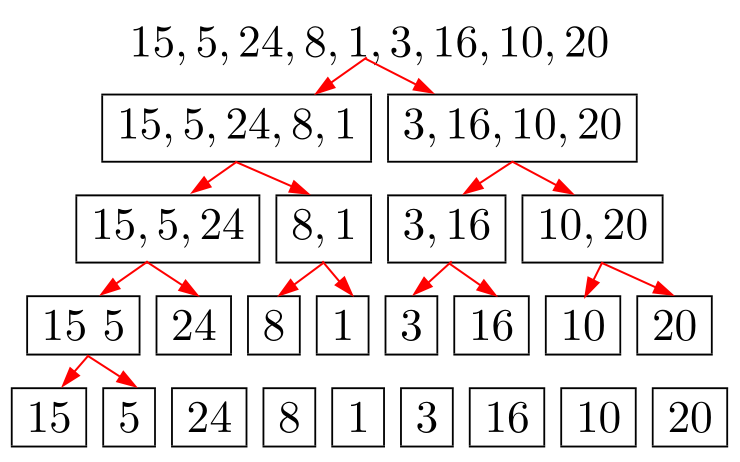
\includegraphics[scale=0.3]{merge-sort1.png}\\
		\end{center}
		Merge:($O(n)$)
		\begin{center}
			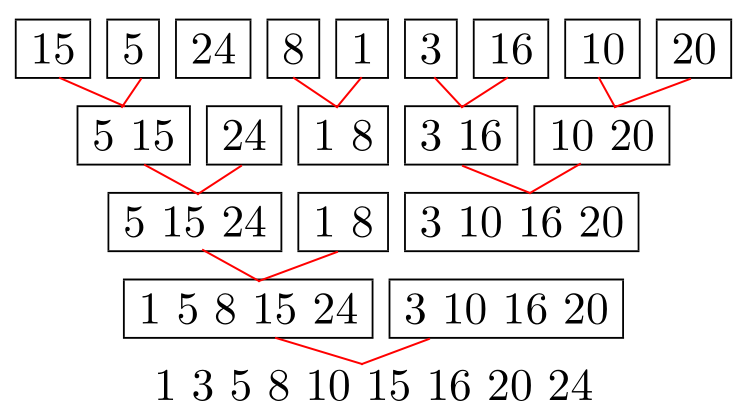
\includegraphics[scale=0.3]{merge-sort2.png}\\
		\end{center}
	\end{eg}

	\subsection{Quick Sort}
	\begin{alg}[Quick sort]
		Like merge sort, quick sort is a divide and conquer algorithm. It picks an element as pivot and partitions the given array around the picked pivot. There are many different versions of quickSort that pick pivot in different ways. It is seen that randomized quicksort works very well in practical cases. 

		After each pass, all elements to the left of the pivot are smaller than the pivot and all elements to the right of the pivot are larger than the pivot, thus the pivot is in the correct position.
		\begin{enumerate}
			\item Select the pivot.
			\item Use the partition method to get the pivot to its correct position.
			\item Repeat this for the subarrays formed to the left and right of the pivot.
	\end{enumerate}
	Time complexities:

	Worst case: $O(n^2)$

	Best and average case: $O(n\log n)$. QuickSort is faster in practice, because its inner loop can be efficiently implemented on most architectures, and in most real-world data. QuickSort can be implemented in different ways by changing the choice of pivot, so that the worst case rarely occurs for a given type of data. However, merge sort is generally considered better when data is huge and stored in external storage. 
	\end{alg}

	\begin{alg}(Partition)
		We will now see how the partition method in quicksort works. Let our pivot be the first element. 
		\begin{enumerate}
			\item Set $p=2,q=n, \text{pivot}=1$. Set ARR$[0]=\-infty,$ ARR$[n+1]=+\infty$.
			\item Until ARR$[p]>$ ARR[pivot], $p=p+1$.
			\item Until ARR$[q]<$ ARR[pivot], $q=q-1$.
			\item If $p<q$, swap(ARR$[p]$,ARR$[q]$). Go to 2.
			\item If $p\geq q$, swap(ARR[pivot],ARR$[q]$). Exit.
	\end{enumerate}
	\end{alg}
	
	\begin{eg}
		Let ARR =$[35,50,15,25,80,20,90,45]$.
		\[\boxed{35},\underbracket{50}_P,15,25,80,20,90,\underbracket{45}_Q\]
		\[\boxed{35},\underbracket{50}_P,15,25,80,\underbracket{20}_Q,90,45\]
		\[\boxed{35},\underbracket{20}_P,15,25,80,\underbracket{50}_Q,90,45\]
		\[\boxed{35},20,15,\underbracket{25}_Q,\underbracket{80}_P,50,90,45\]
		\[25,20,15,\boxed{35},80,50,90,45\]
	\end{eg}

	\subsection{Comparison of sorting algorithms}
		\begin{center}
			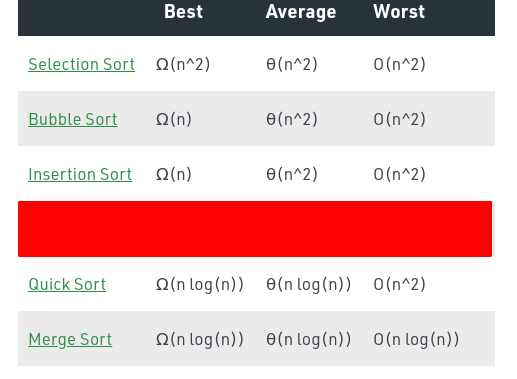
\includegraphics[scale=0.7]{sort.png}\\
		\end{center}


	\section{Stack}
	Stacks are a kind of data structure where we are only interested in the last inserted element at any point of time. It is a LIFO(Last In First Out) data structure. The last inserted element is called the TOP. A stack can be implemented by an array or a linked list.
	\[1\ 9\ 3\ 8\ 5\leftarrow\boxed{\text{top}}\]
	\subsection{Push}
	\begin{alg}[Push]
		Push is a stack operation that inserts an element to the top of the stack.
		\begin{enumerate}
			\item Set TOP = TOP + 1
			\item Set STACK[TOP] = VALUE. Exit.
	\end{enumerate}
	\end{alg}
	\subsection{Pop}
	\begin{alg}[Pop]
		The pop operation removes the top element from the stack and returns its value.
		\begin{enumerate}
			\item Set VALUE = STACK[TOP]
			\item Set TOP = TOP - 1.
			\item Return VALUE. Exit.
	\end{enumerate}
	There is an operation similar to POP where we only return the value of the TOP element but do not change the TOP pointer. It is called \textbf{PEEK}.
	\end{alg}

	All operations take $O(1)$ time(even for linked list implementation).

	\subsection{Evaluation of expressions}
	Generally, we write an arithmetic expression in its \textbf{infix} form where the operator lies between the operands. However, such an expresstion cannot be computed from left to right(or, right to left) due to the precedence of operators. Thus, we convert it into \textbf{postfix} form for such computations. A stack is used for this purpose.
	\begin{alg}[Infix to Postfix]
		Suppose Q is an arithmetic expression written in infix notation. This algorithm finds the equivalent postfix expression P.
		\begin{enumerate}
			\item Push `(' onto STACK, and add `)' to the end of Q. Scan Q from left to right and repeat the following steps.
			\item If STACK is empty, exit. P is the required postfix expression.
			\item If an operand is encountered, add it to P.
			\item  If a left parenthesis is encountered, push it onto STACK.
			\item  If an operator $\circ$ is encountered,
				\begin{enumerate}
					\item Repeatedly pop from STACK and add to P each operator (on the top of STACK) which has the same precedence as or higher precedence than $\circ$.
					\item Add $\circ$ to STACK.
			\end{enumerate}
			
			\item If a right parenthesis is encountered,
				\begin{enumerate}
					\item Repeatedly pop from STACK and add to P each operator (on the top of STACK) until a left parenthesis is encountered.
					\item Remove the left parenthesis from the STACK.
			\end{enumerate}
	\end{enumerate}
	\end{alg}
	\begin{alg}[Evaluation of postfix expression]
		Now that we have converted our infix to postfix, we would like to evaluate the expression.
		\begin{enumerate}
			\item Add a right parenthesis ) at the end of P. Scan P from left to rightand repeat the following steps.
			\item If only a ) is left to be scanned in P, exit. VALUE = STACK[TOP].
			\item If an operand is encountered, put it on STACK.
			\item If an operator $\circ$ is encountered,
				\begin{enumerate}
					\item Pop the two top elements of STACK, where A is the top element and B is the next-to-top element.
					\item Evaluate B $\circ$ A and push the result into the stack.

			\end{enumerate}
	\end{enumerate}
	\end{alg}
	

	\section{Queue}
	Like Stack, Queue is a linear structure which follows a particular order in which the operations are performed. The order is First In First Out (FIFO).
	\[\boxed{\text{front}}\to1\ 9\ 3\ 8\ 5\leftarrow\boxed{\text{rear}}\]

	\subsection{Salient Features}
	\begin{itemize}
		\item Both insertion and deletion is done in $O(1)$ time.
		\item Array implementation is often problematic for large number of enque and deque operations. So, we may use linked list(time complexity remains same).
		\item We often use \textbf{circular queues} for better utilisation of space. Also, we only need to have a pointer for the front/rear as the other is always next to it.
		\item We can \textbf{implement a queue using stack}. We will require two stacks. We can also \textbf{implement a stack using queue}. We will need two queues.
	\end{itemize}
	\subsection{Enque}
	\begin{alg}[Enque]
		Insert element to the REAR.
		\begin{enumerate}
			\item Set REAR = REAR + 1
			\item Set QUEUE[REAR] = VALUE. Exit.
	\end{enumerate}
	\end{alg}
	\subsection{Deque}
	\begin{alg}[Deque]
		Remove element from the FRONT and return its value.
		\begin{enumerate}
			\item Set VALUE = QUEUE[FRONT]
			\item Set FRONT = FRONT + 1. Exit.
	\end{enumerate}
	\end{alg}
	
	\subsection{Priority Queue}
	\begin{defn}[Priority queue]
		Priority Queue is an extension of queue with following properties.
		\begin{enumerate}
			\item Every item has a priority associated with it.
			\item An element with high priority is dequeued before an element with low priority.
			\item If two elements have the same priority, they are served according to their order in the queue.
	\end{enumerate}
	It is often implemented using heaps.
	\end{defn}

	\section{Binary Tree}
	Until  now, we have only studied \textbf{linear data structures}. Trees are \textbf{hierarchical data structures}.
	\begin{defn}[Root, children, parent, sibling, leaf, edge]
		The topmost node is called root of the tree. The elements that are directly under an element are called its children. The element directly above something is called its parent. Two nodes with the same parent are called siblings. A node that has no children is called a leaf node. All other nodes(except root) are called edges.
	\end{defn}
	
	\begin{defn}[Level or depth]
		The number of edges on the path from the root to a node is called its level or depth. The root, unless mentioned otherwise, is at level 1.
	\end{defn}

	\begin{defn}[Height]
		Height of a tree is the maximum level for any node in the tree.
	\end{defn}
	\begin{defn}[Binary tree]
		A tree where each node has at most 2 children. These are called the left child and the right child.
	\end{defn}
	\subsection{Salient features}
	\begin{itemize}
		\item The maximum number of nodes at level $l$ of a binary tree is $2^l$. 
		\item The maximum number of nodes in a binary tree of height $h$ is $2^h-1$.
		\item In a binary tree with $n$ nodes, minimum possible height is $\log_2(n+1)$.
		\item A binary tree with $L$ leaves has at least $\lceil\log_2L\rceil+1$ levels.
		\item In binary tree where every node has 0 or 2 children, the number of leaf nodes is always one more than nodes with two children.
		\item Insertion and deletion has no rules except the maximum of 2 children. This is can be done really fast. This is faster than arrays but slower than linked lists.
		\item Searching items in a general binary tree is slow. As there is no particular order, every node may have to be checked in the worst case. 
	\end{itemize}
	\subsection{Types of binary trees}
	\begin{defn}[Full binary tree]
		Every node has 0 or 2 children.
	\end{defn}
	\begin{defn}[Complete binary tree]
		All the levels are completely filled except possibly the last level and the last level has all keys as left as possible. 
	\end{defn}
	\begin{defn}[Perfect binary tree]
		All the internal nodes have two children and all leaf nodes are at the same level. 
	\end{defn}
	\begin{defn}[Balanced binary tree]
		$h=O(\log n)$
	\end{defn}
	\begin{defn}[Degenrate binary tree]
	Every internal node has one child.
	\end{defn}
	\subsection{Traversal}
	Unlike linear data structures which have only one logical way to traverse them, trees can be traversed in different ways.
	\begin{itemize}
		\item Inorder: Left, Root, Right
		\item Preorder: Root, Left, Right
		\item Postorder: Left, Right, Root
		\item Level order: Each level, left to right
	\end{itemize}
	All traversals can be done in $O(n)$ time. The first three are called depth-first traversals. The inorder traversal along with any other depth-first traversal can be used to recontruct a binary tree.
	\subsection{Threading}
	A binary tree is made threaded by making all right child pointers that would normally be NULL, point to the inorder successor of the node (if it exists). The idea of threaded binary trees is to make inorder traversal faster and do it without stack and without recursion.

	\section{Binary Search Tree}
	As the name suggests, a binary search tree is a form of binary tree that makes searching easier. We lose some time in insertion and deletion.

	\begin{defn}[Binary search tree]
		A binary tree with following rules:
		\begin{enumerate}
			\item The left subtree of a node contains only nodes with keys lesser than the node’s key.
			\item The right subtree of a node contains only nodes with keys greater than the node’s key.
			\item The left and right subtree each must also be a binary search tree. 
	\end{enumerate}
	\end{defn}
	Searching, insertion and deletion all have a complexity of $O(h)$. In the worst case, this is $O(n)$.
	\subsection{Searching}
	Searching in BST is faster than unordered linked lists but slower than arrays.\\
	\begin{alg}
	bstSearch(tree, VALUE):
	\begin{enumerate}
		\item Set NODE = ROOT.
		\item If NODE is NULL, exit. VALUE not found.
		\item If NODE.key = VALUE, VALUE found at NODE. Exit.
		\item If VALUE $<$ NODE.key, bstSearch(left subtree, VALUE).
		\item If VALUE $>$ NODE.key, bstSearch(right subtree, VALUE).
\end{enumerate}
	\end{alg}
	\begin{eg}
		Let the BST be:
		\begin{center}
			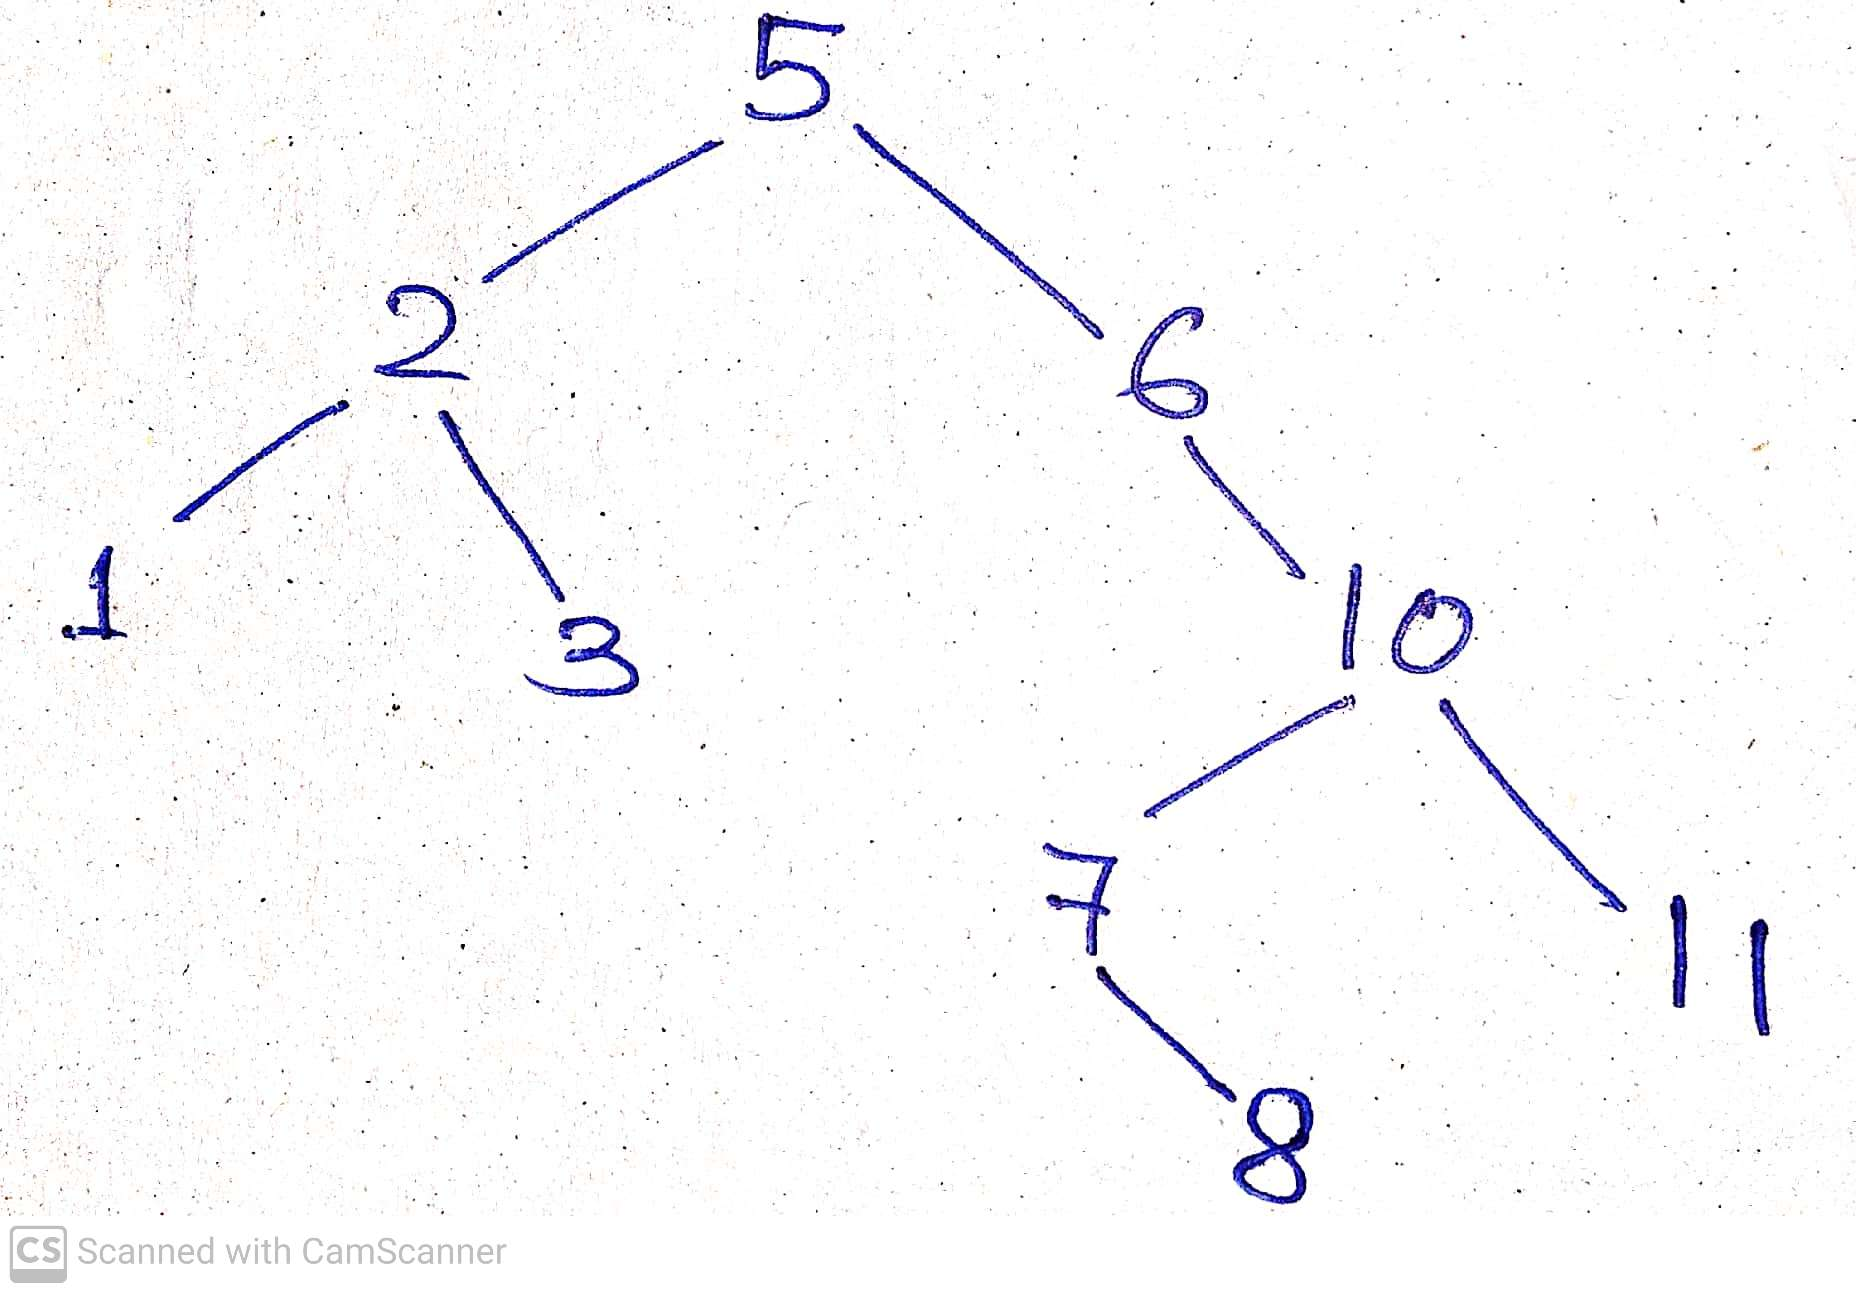
\includegraphics[scale=0.07]{bst1.jpg}\\
		\end{center}
		The search of the key 7 happens like:
		\begin{center}
			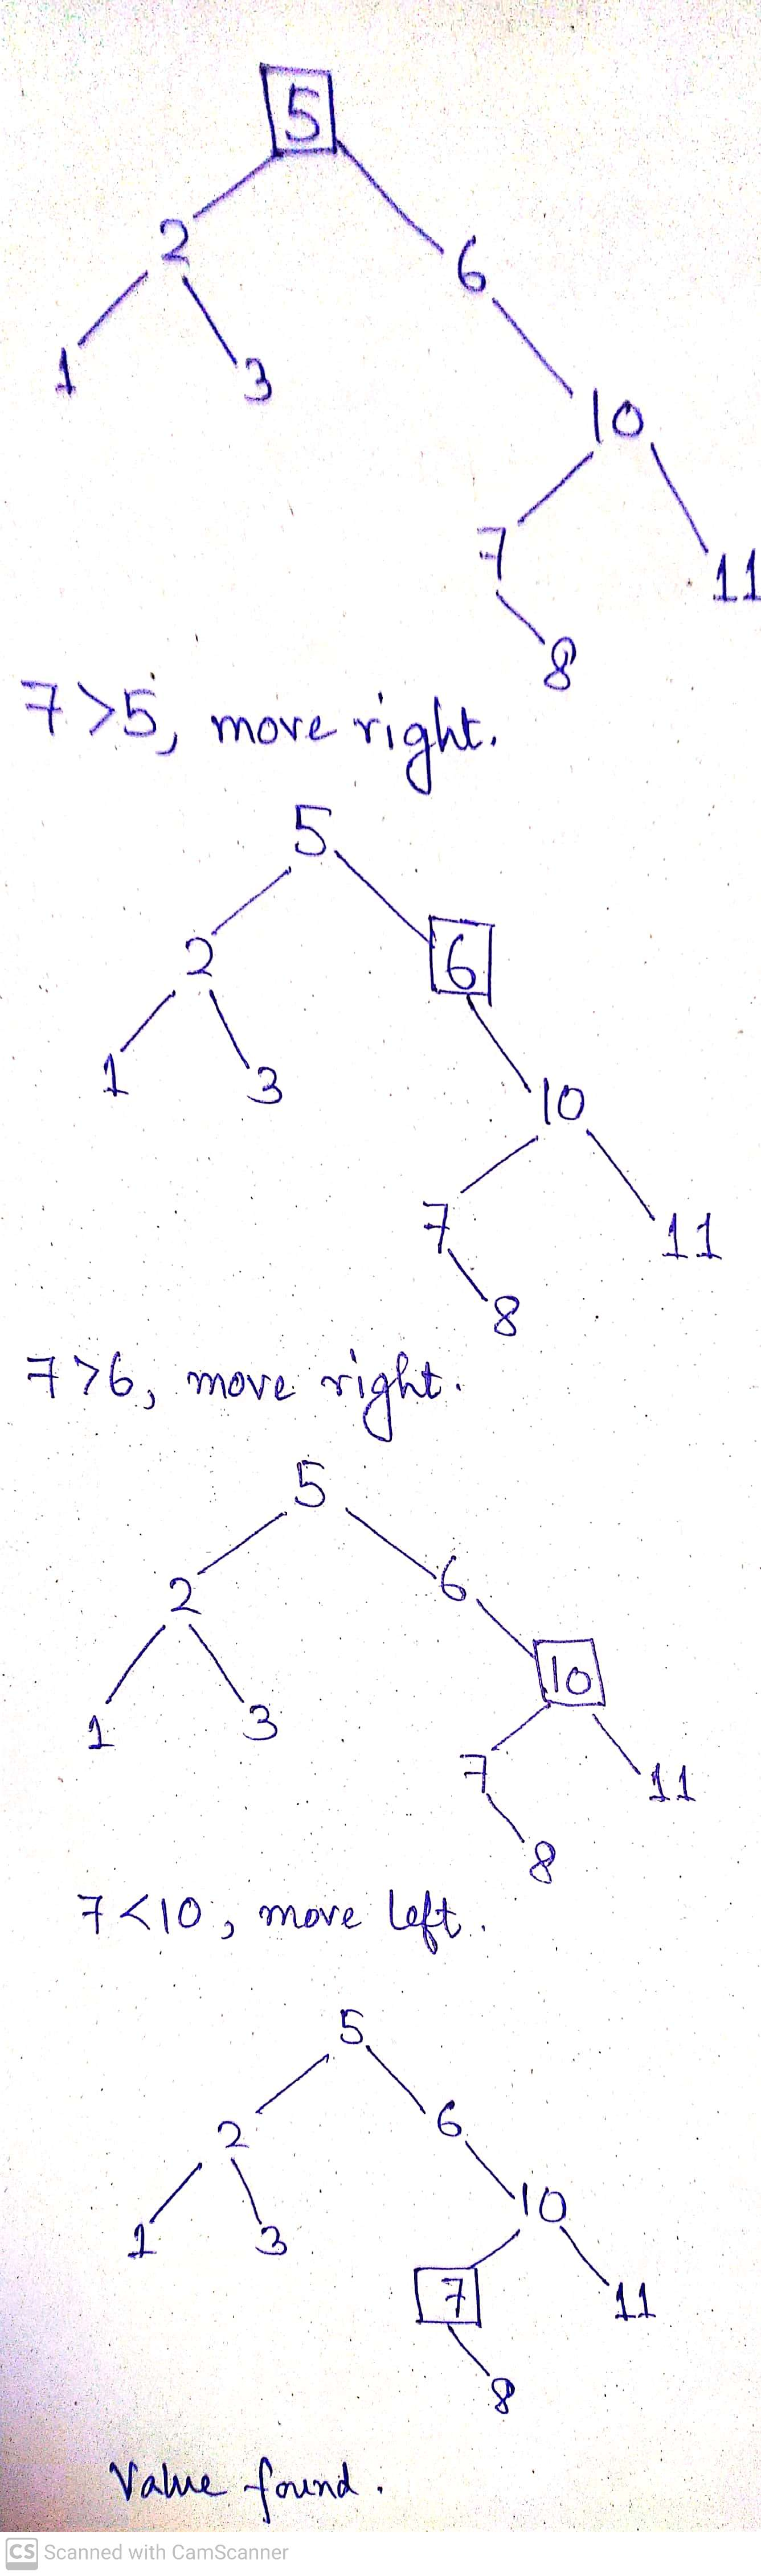
\includegraphics[scale=0.1]{bst2.jpg}\\
		\end{center}
	\end{eg}
	\subsection{Insertion}
	\begin{alg}\hfill\\
		insert(tree, VALUE)
		\begin{enumerate}
			\item Set NODE = ROOT.
			\item If NODE = NULL, set NODE.key = VALUE. Set NULL as NODE's as its children. Exit.
			\item If VALUE $<$ NODE.KEY, insert(left subtree, VALUE)
			\item If VALUE $>$ NODE.KEY, insert(right subtree, VALUE)
	\end{enumerate}
	\end{alg}
	\begin{eg}
		Let the BST be:
		\begin{center}
			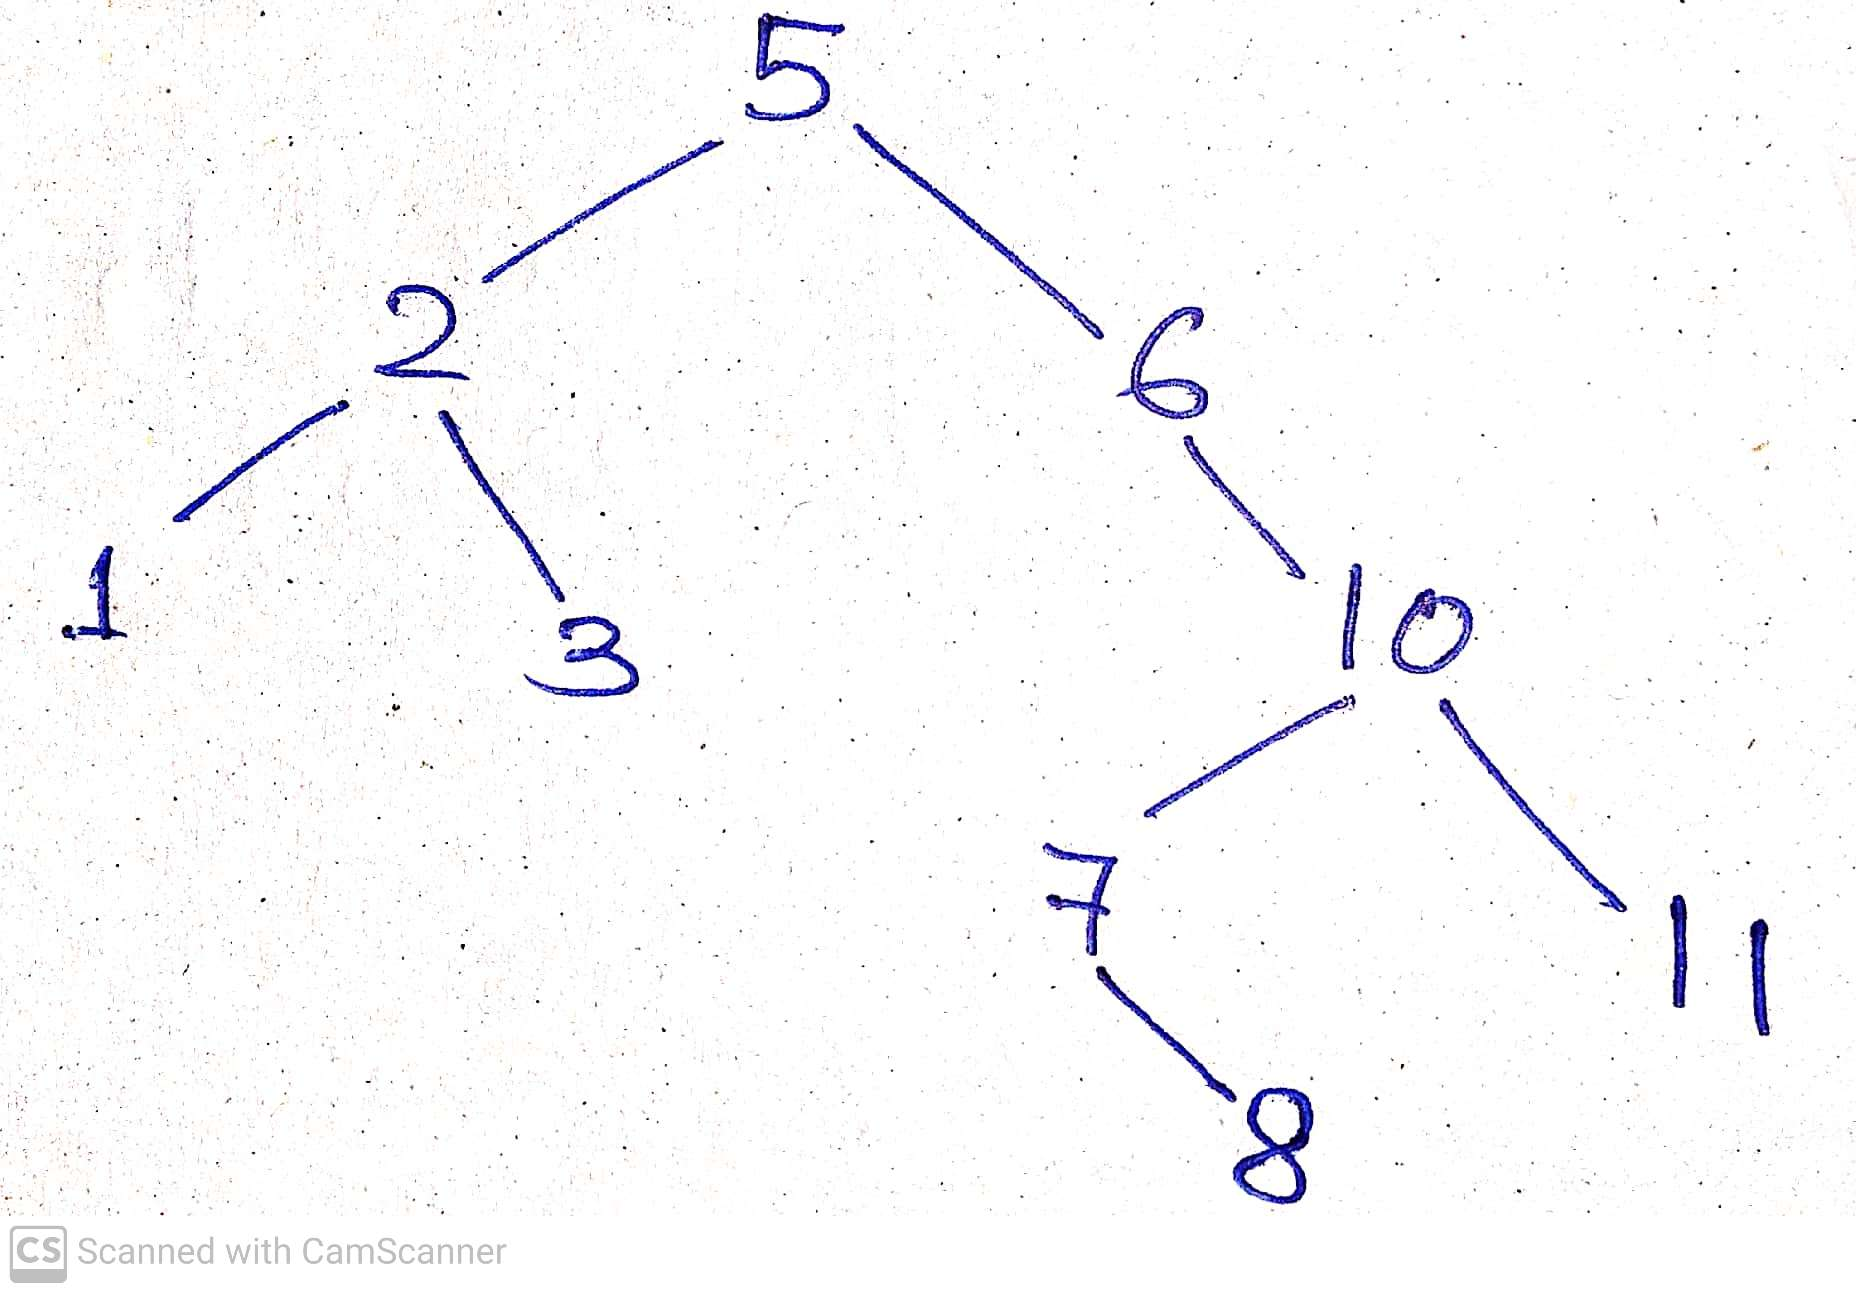
\includegraphics[scale=0.07]{bst1.jpg}\\
		\end{center}
		We need to insert 4.
		\begin{center}
			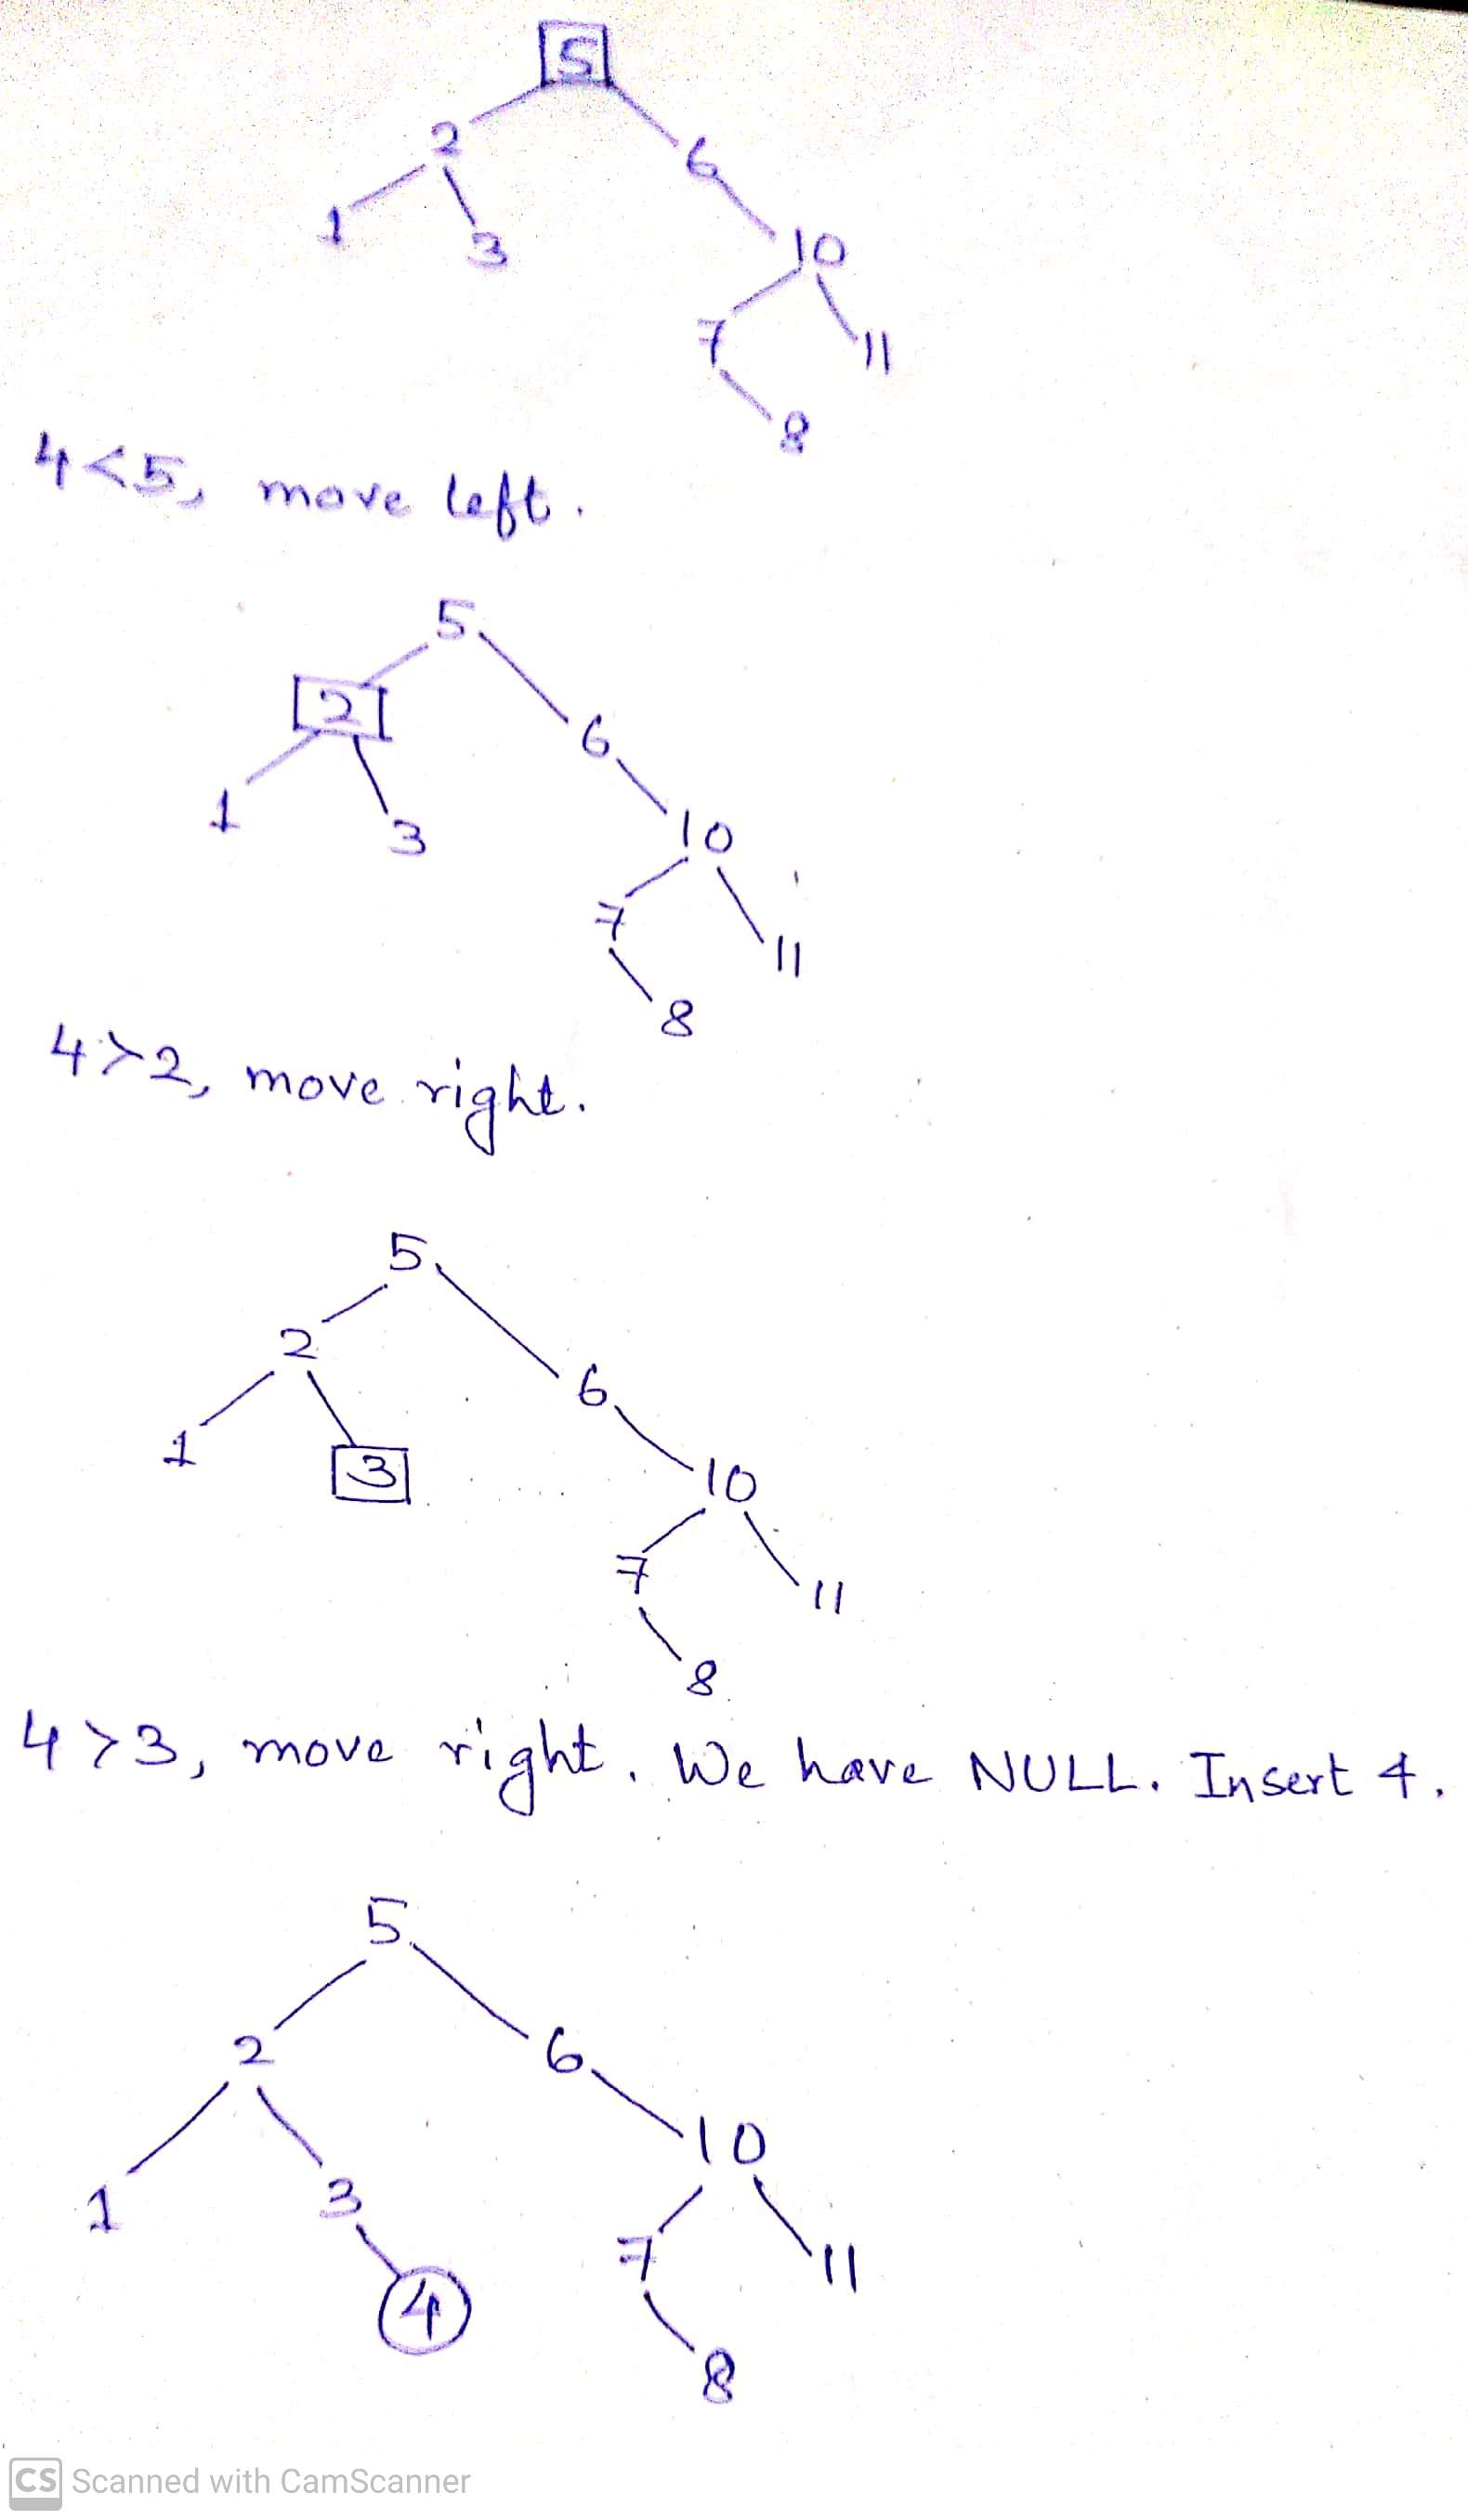
\includegraphics[scale=0.16]{bst3.jpg}\\
		\end{center}
	\end{eg}

	\begin{eg}
		We have to insert a given list of numbers in order.
		\begin{center}
			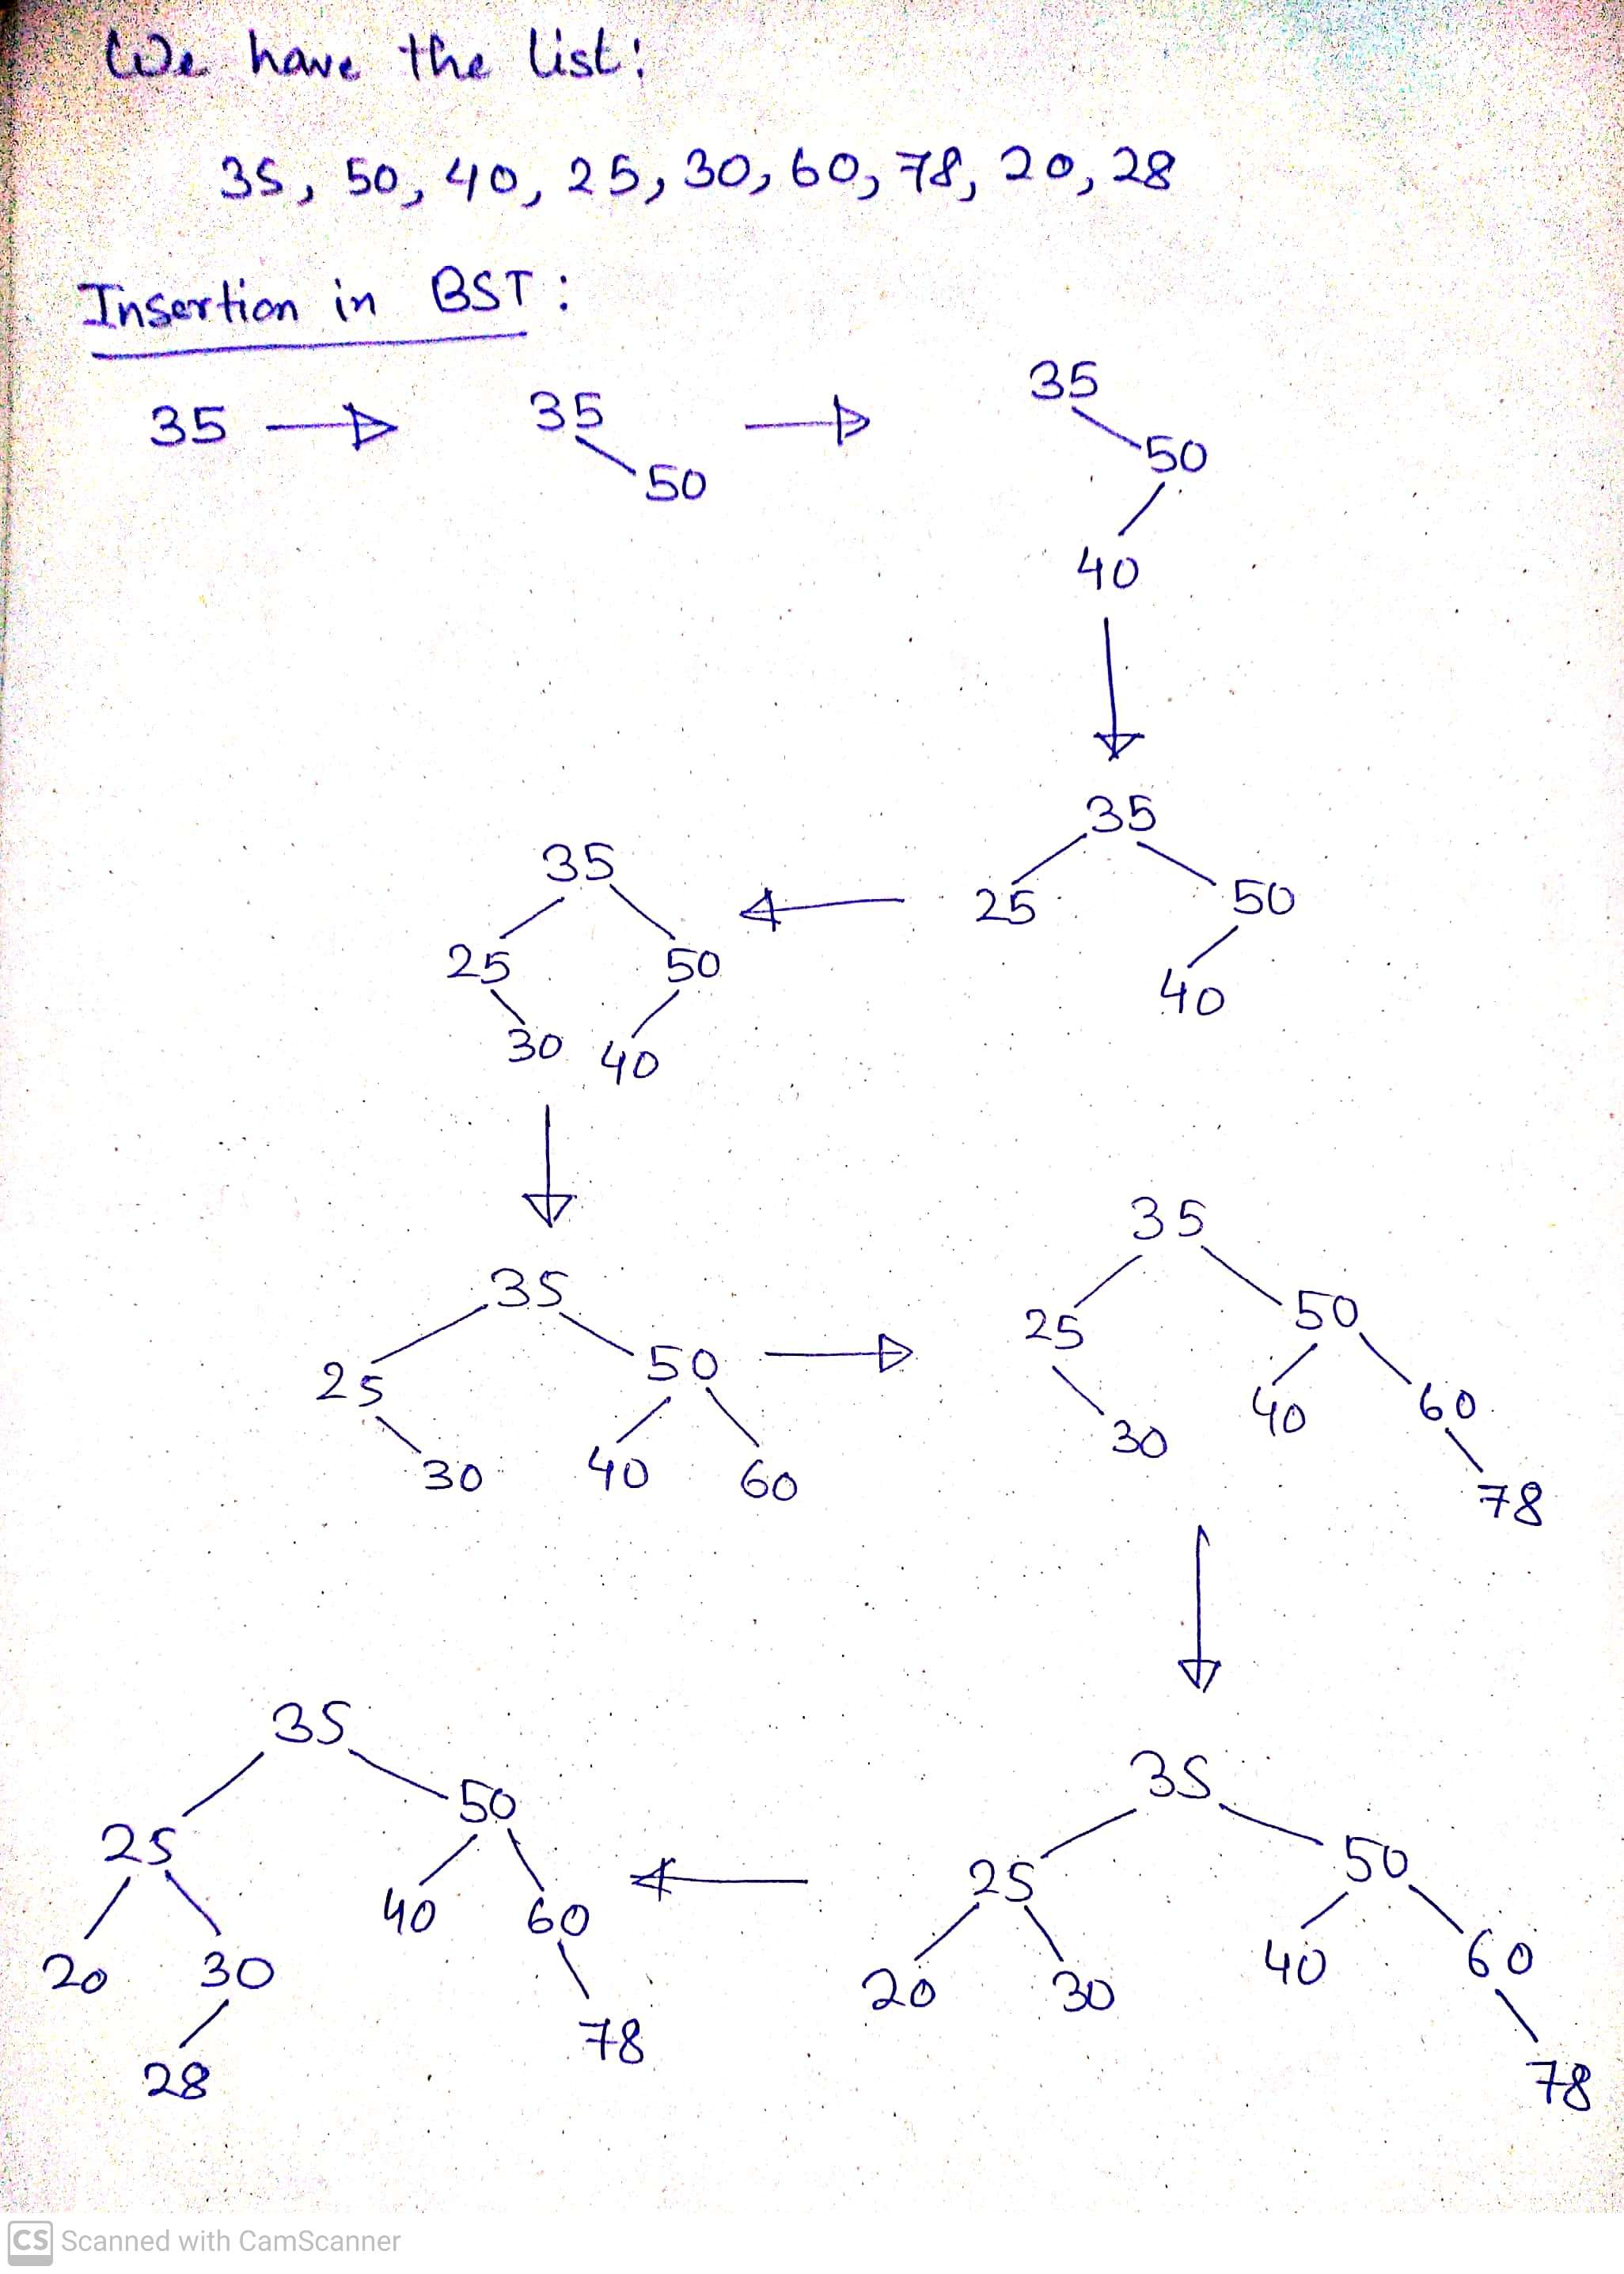
\includegraphics[scale=0.1]{bst4.jpg}\\
		\end{center}
	\end{eg}
	\subsection{Deletion}
	\begin{alg}\hfill
		\begin{itemize}
			\item If node to be deleted is the leaf: Simply remove from the tree. 
			\item If node to be deleted has only one child: Copy the child to the node and delete the child.
			\item If node to be deleted has two children: Find inorder successor of the node. Copy contents of the inorder successor to the node and delete the inorder successor. Note that inorder predecessor can also be used. 
		\end{itemize}
	\end{alg}

	\subsection{AVL Search Tree}
	As we have seen, all the algorithms require $O(h)$ time. Thus, we would like to reduce the height of a tree as much as possible.
	\begin{defn}[Balance factor]
		The balance factor of a node is given by
		\[\text{Balance factor}=h(\text{left subtree})-h(\text{right subtree})\]
	\end{defn}
	\begin{defn}[AVL search tree]
		A balanced binary search tree(i.e., $h=O(\log n)$) such that the balance factor of each node is in the set $\{-1,0,1\}$.
	\end{defn}

	AVL search trees can be used when we need to do a lot of searching but insertion and deletion are not done frequently.

	\subsubsection{Balancing}
	We have 4 types of unbalancedness in a BST.\\
	LL and RR only require 1 rotation to balance.
		\begin{center}
			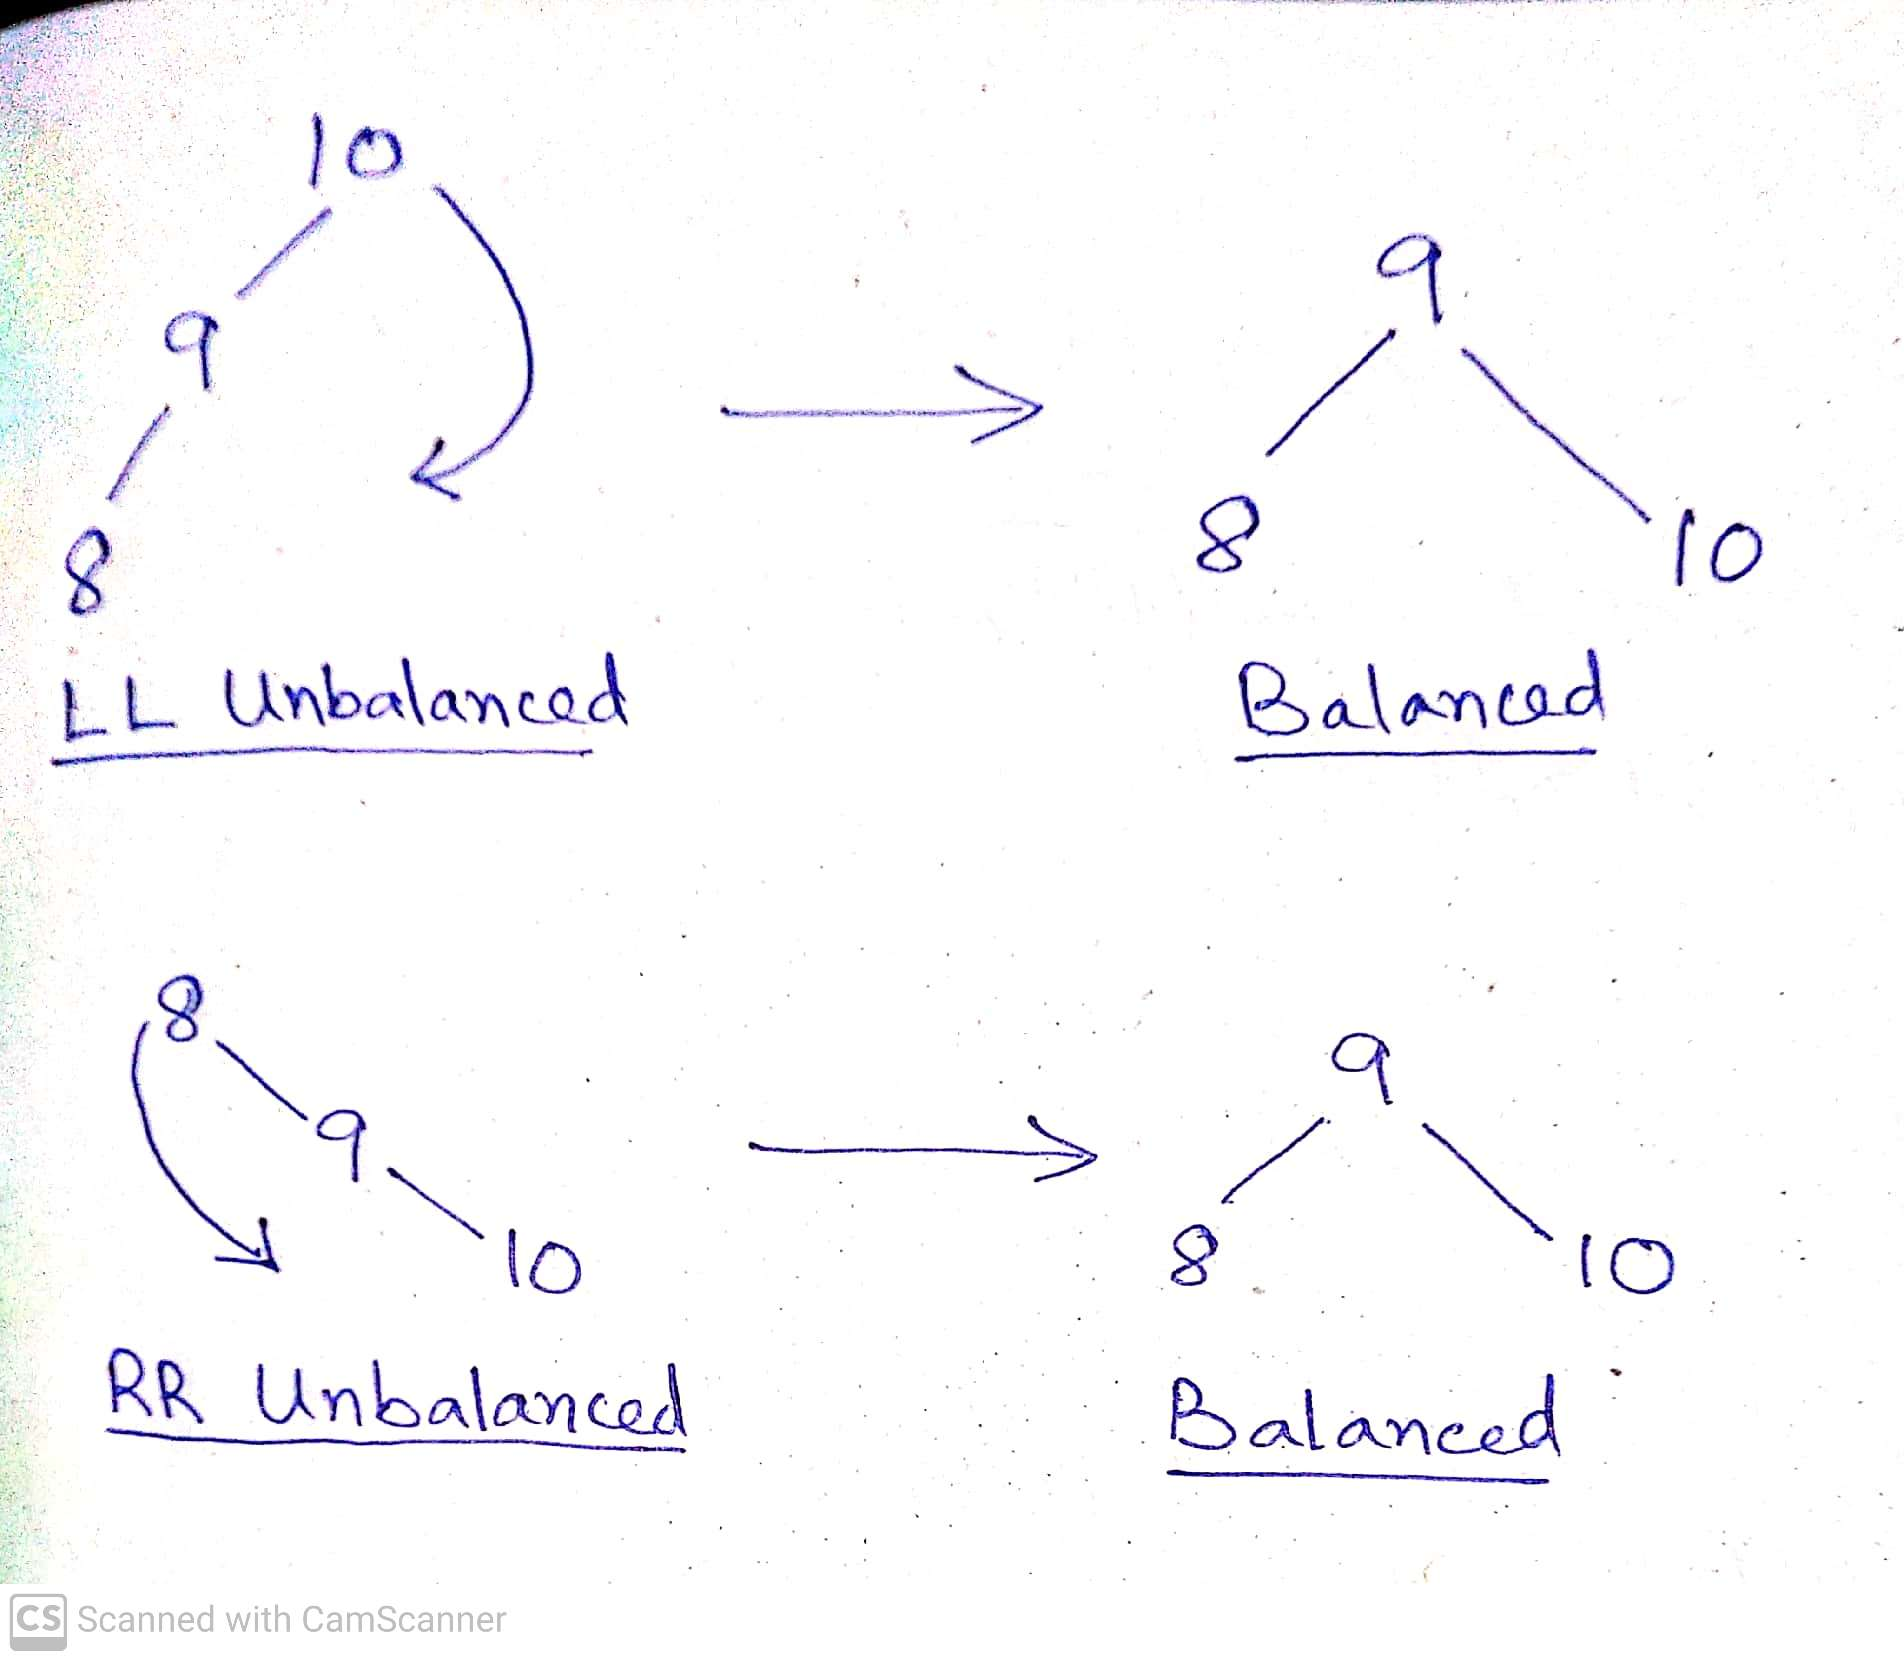
\includegraphics[scale=0.09]{LL-RR.jpg}\\
		\end{center}
		LR and RL first need to be converted to LL and RR, respectively. Thus, they require 2 rotations to balance.
		\begin{center}
			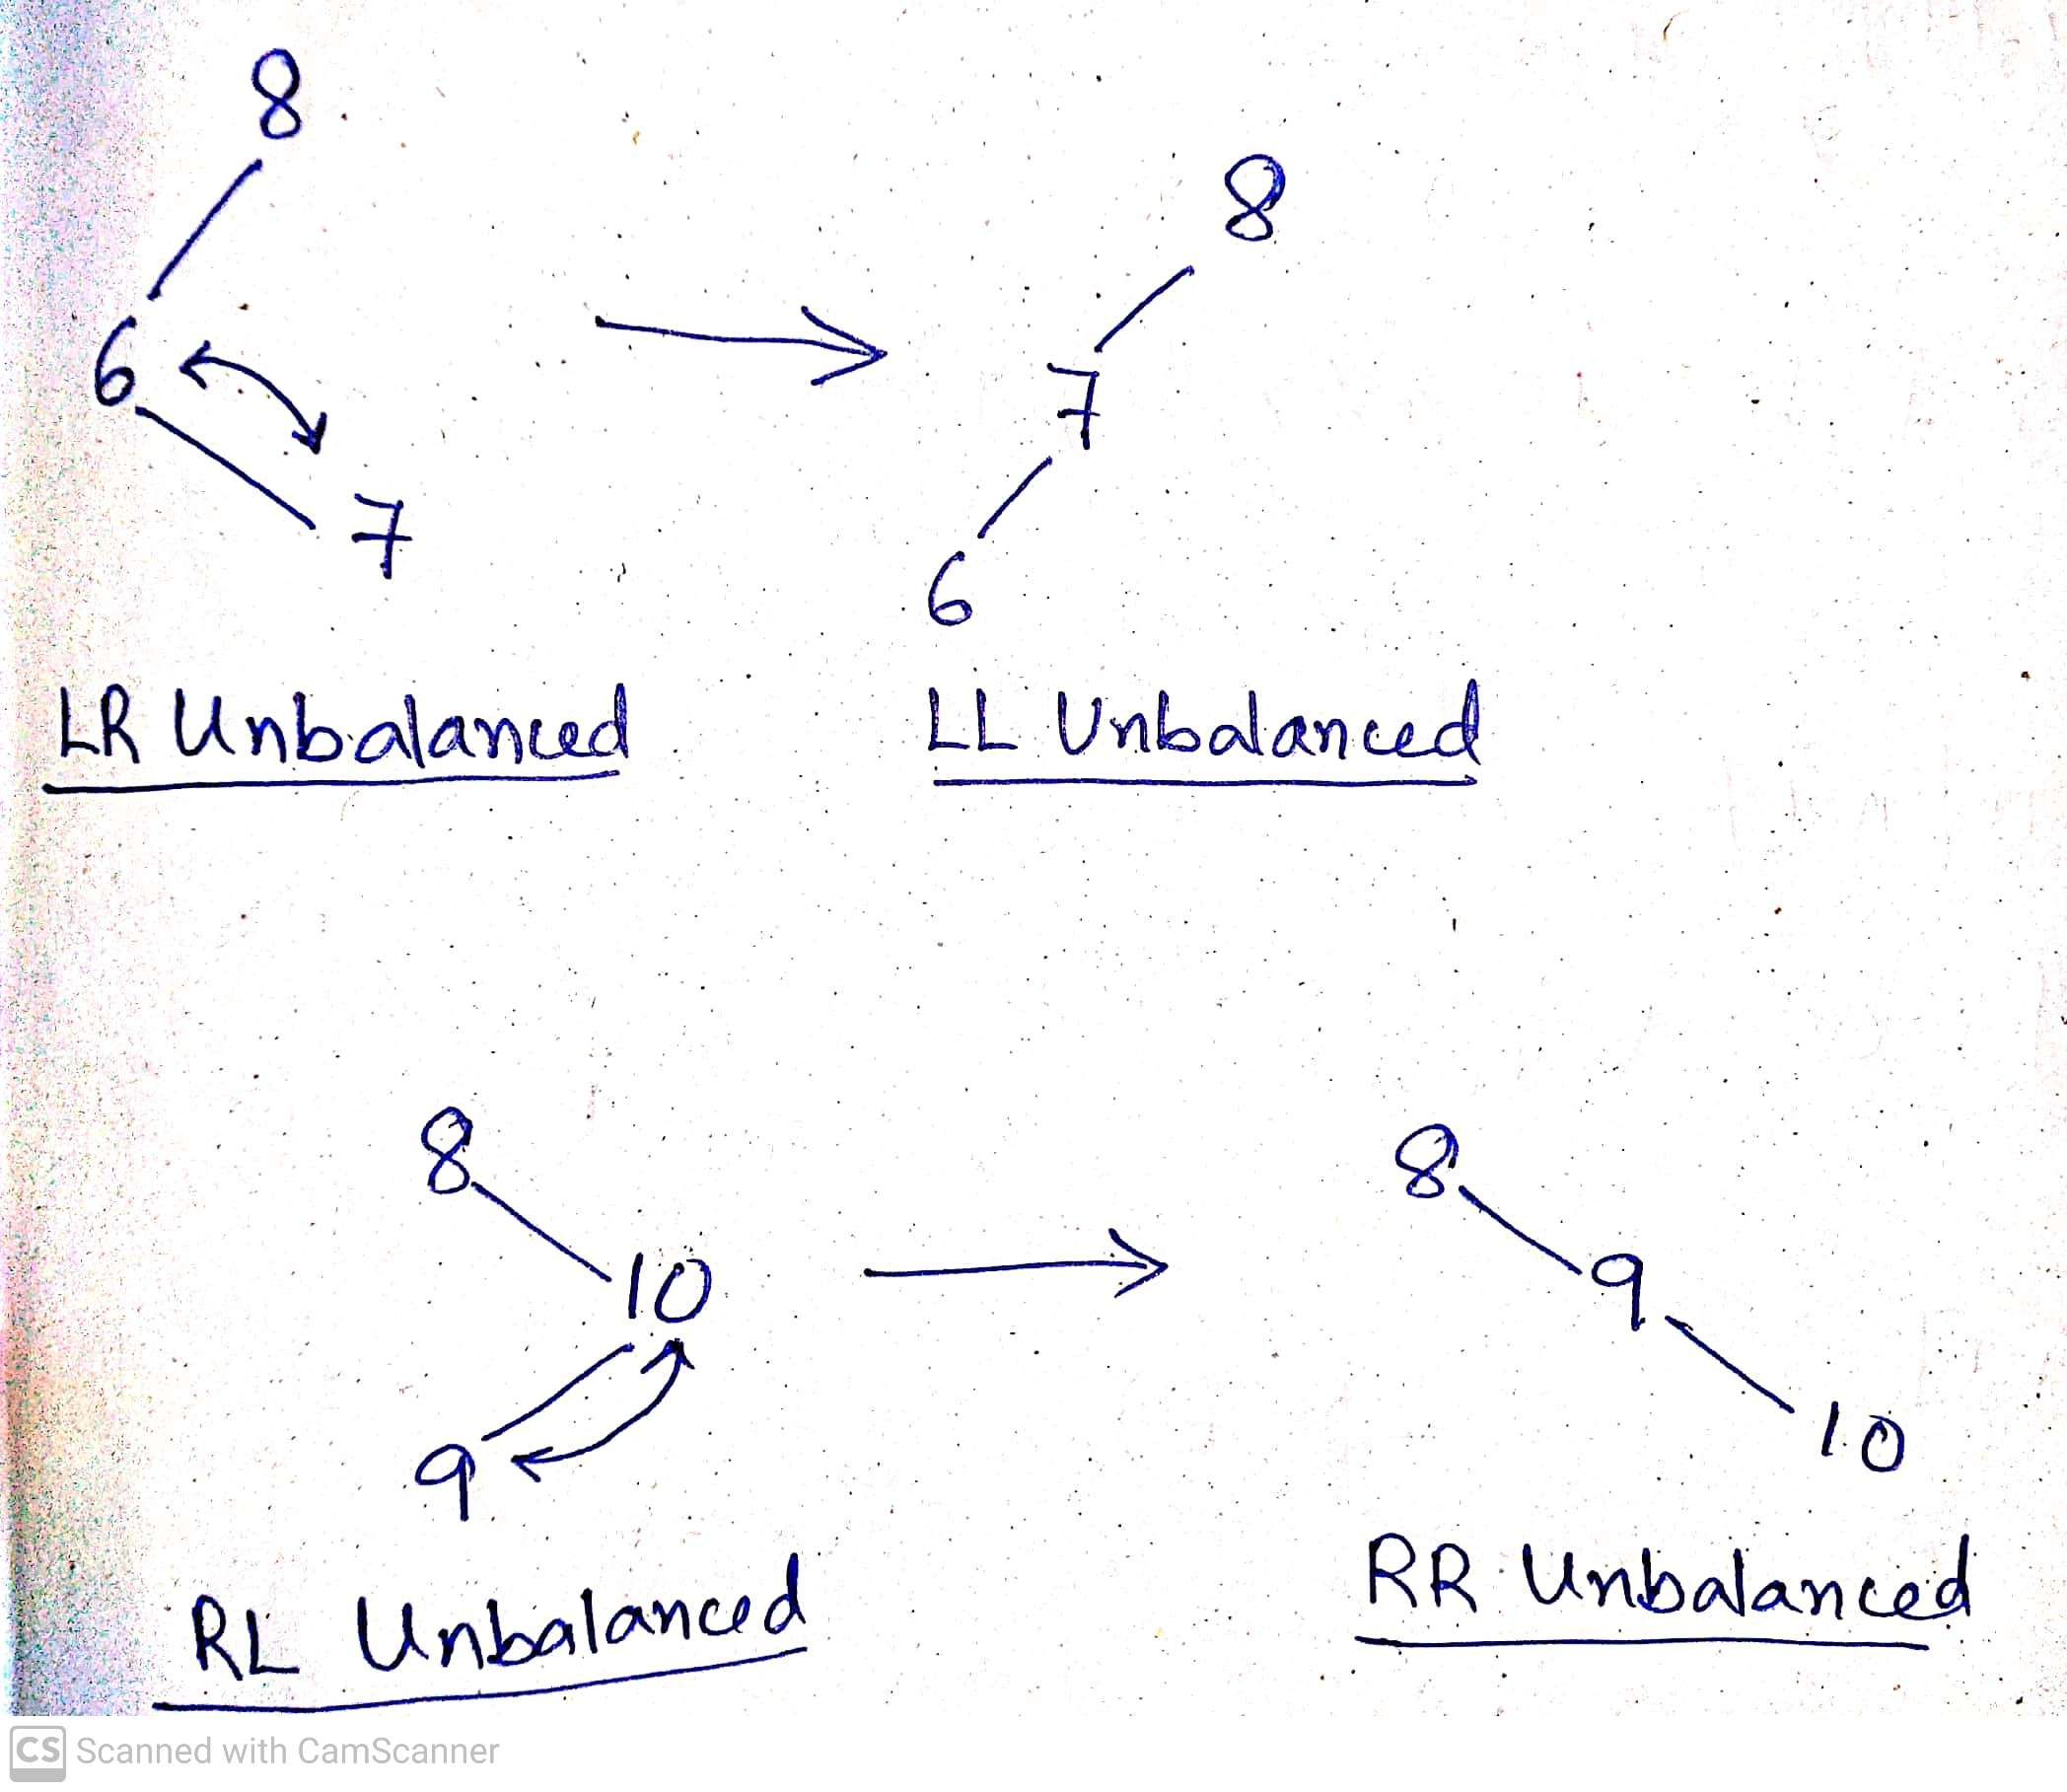
\includegraphics[scale=0.08]{LR-RL.jpg}\\
		\end{center}

		So, how do we balance
		\begin{center}
			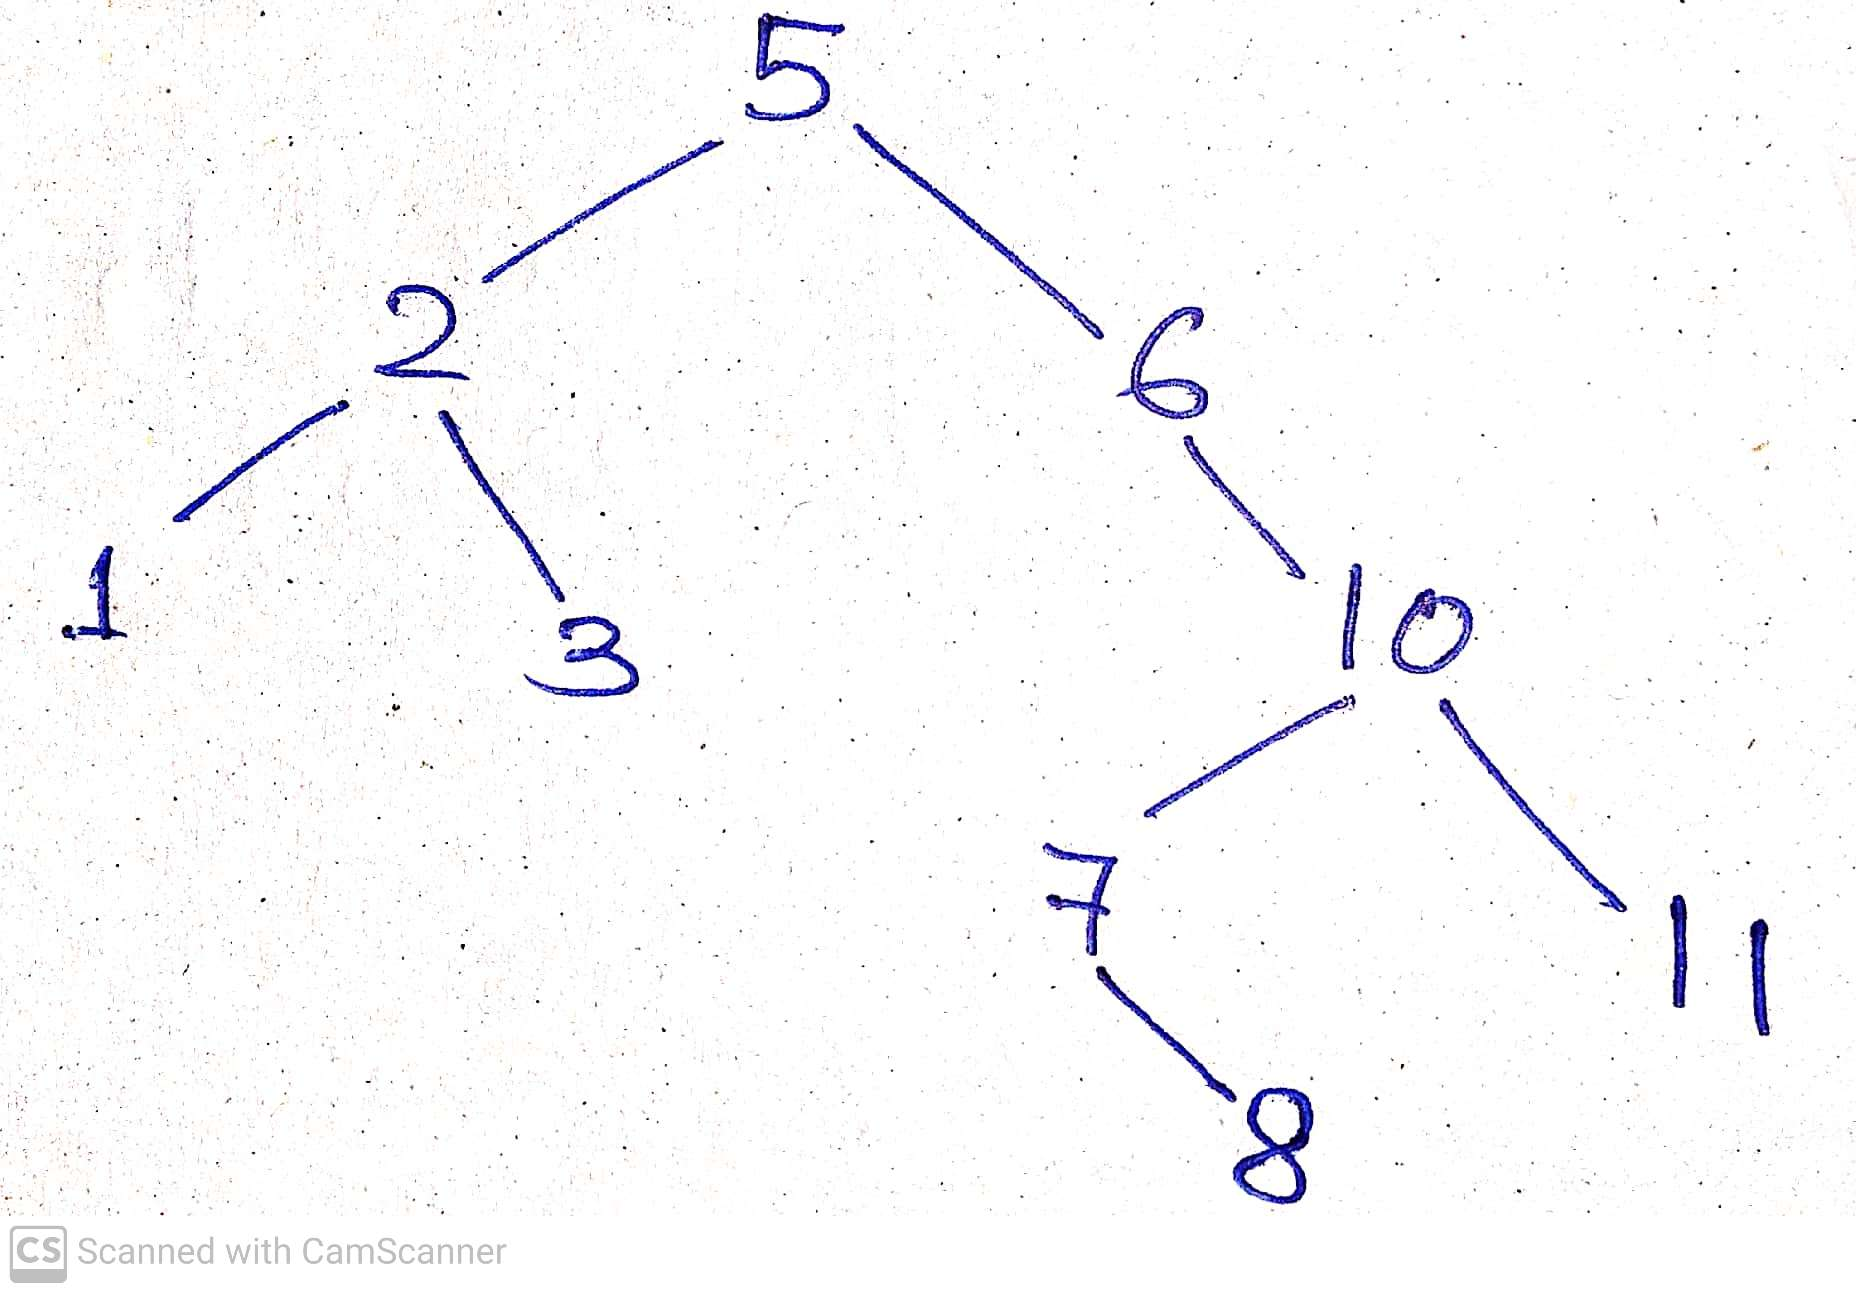
\includegraphics[scale=0.08]{bst1.jpg}\\
		\end{center}
		We note down the balance factor of each node. Leaf nodes always have a balnce factor of 0.

		\begin{center}
			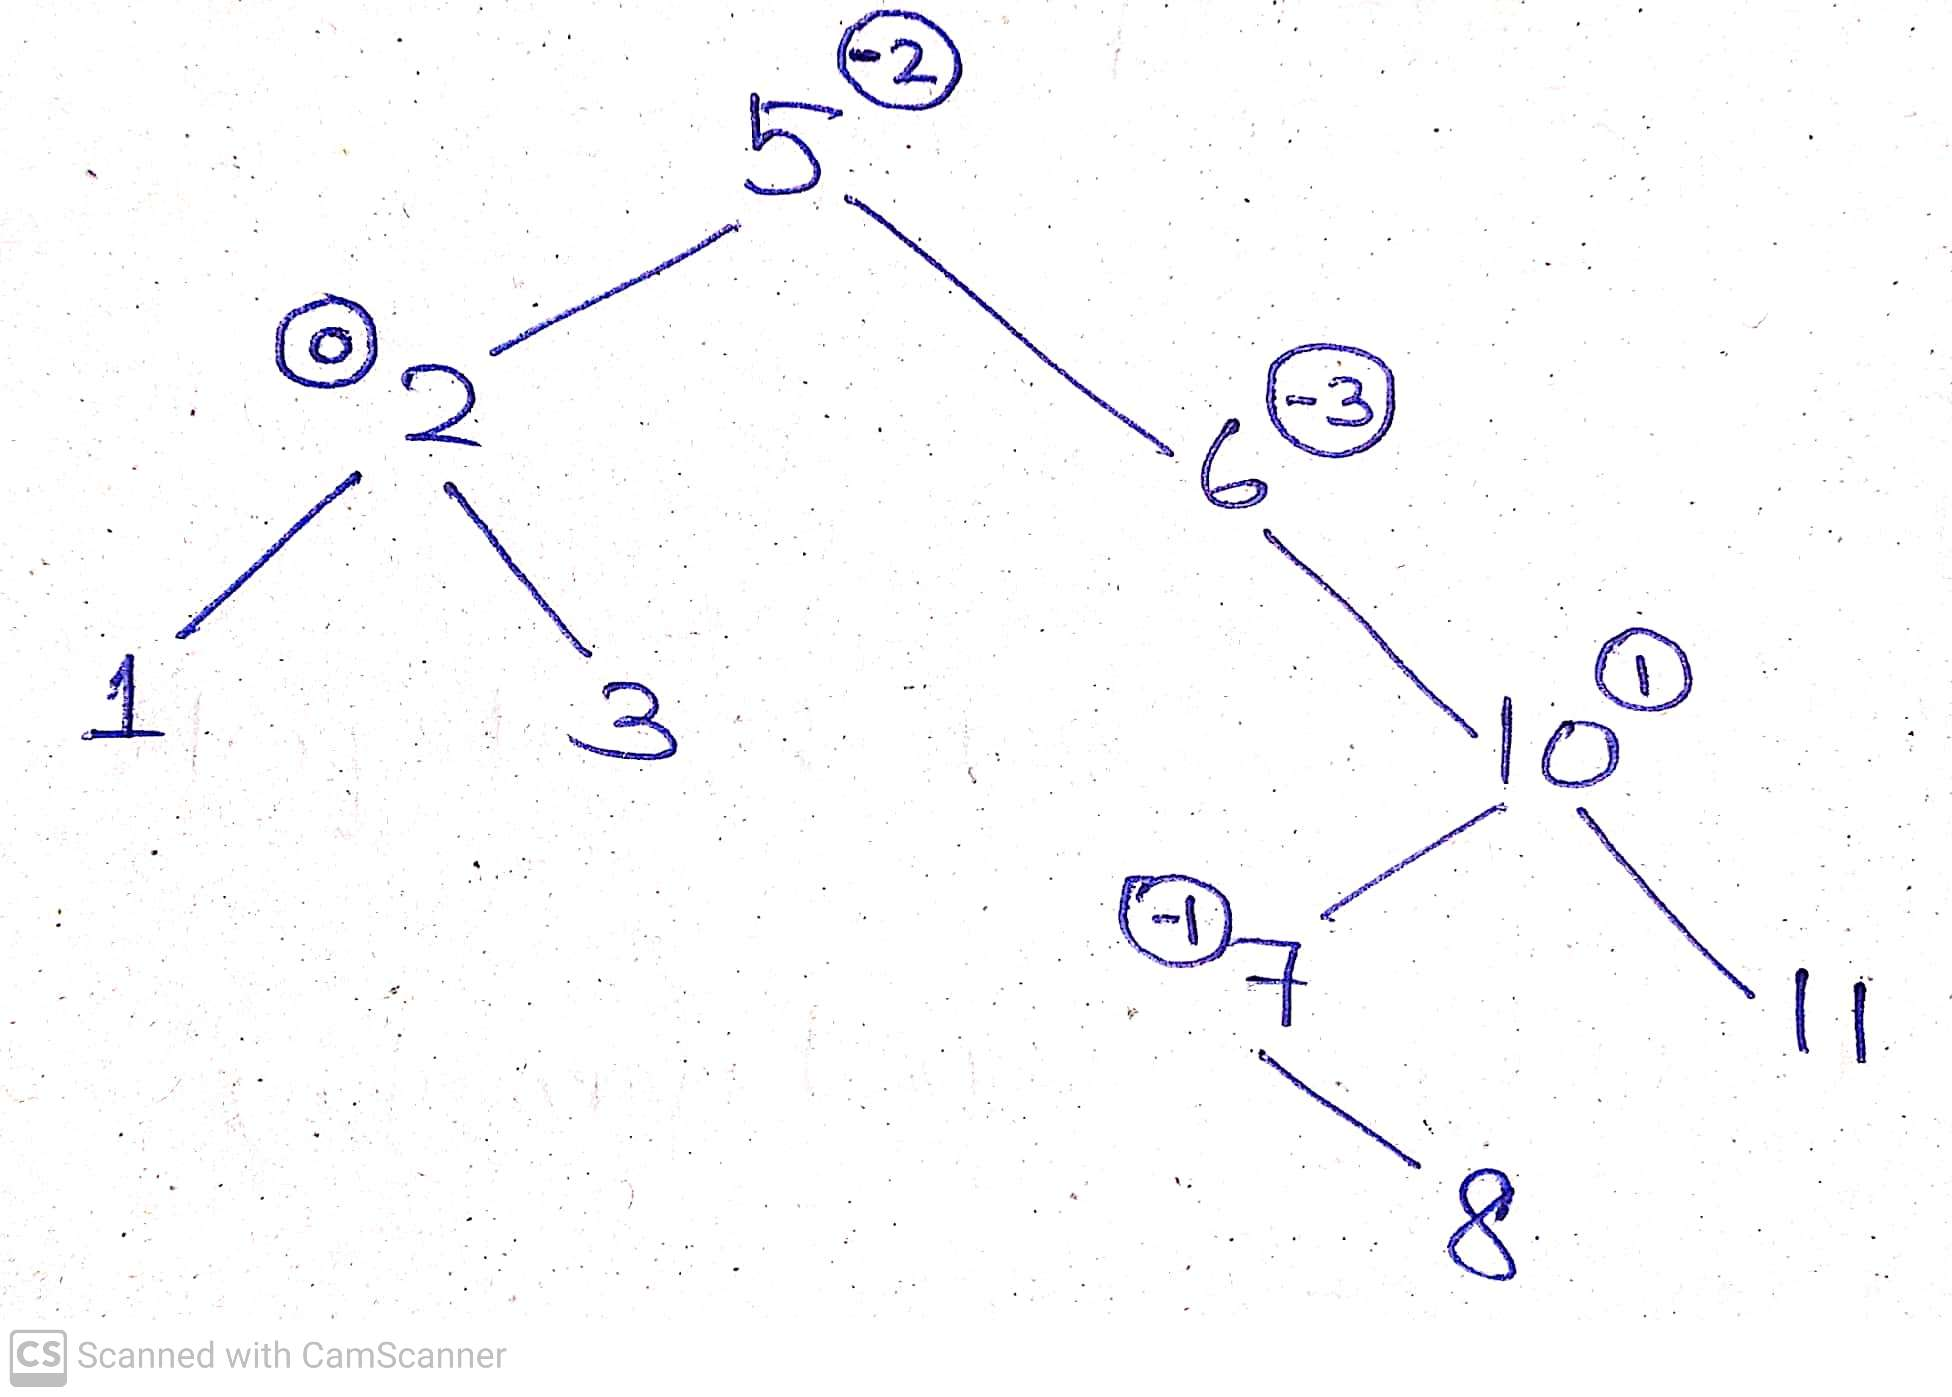
\includegraphics[scale=0.1]{balance1.jpg}\\
		\end{center}
		Clearly the BST is unbalanced. We want to convert it to an AVL search tree.\\
		We perform the following rotations.
		\begin{center}
			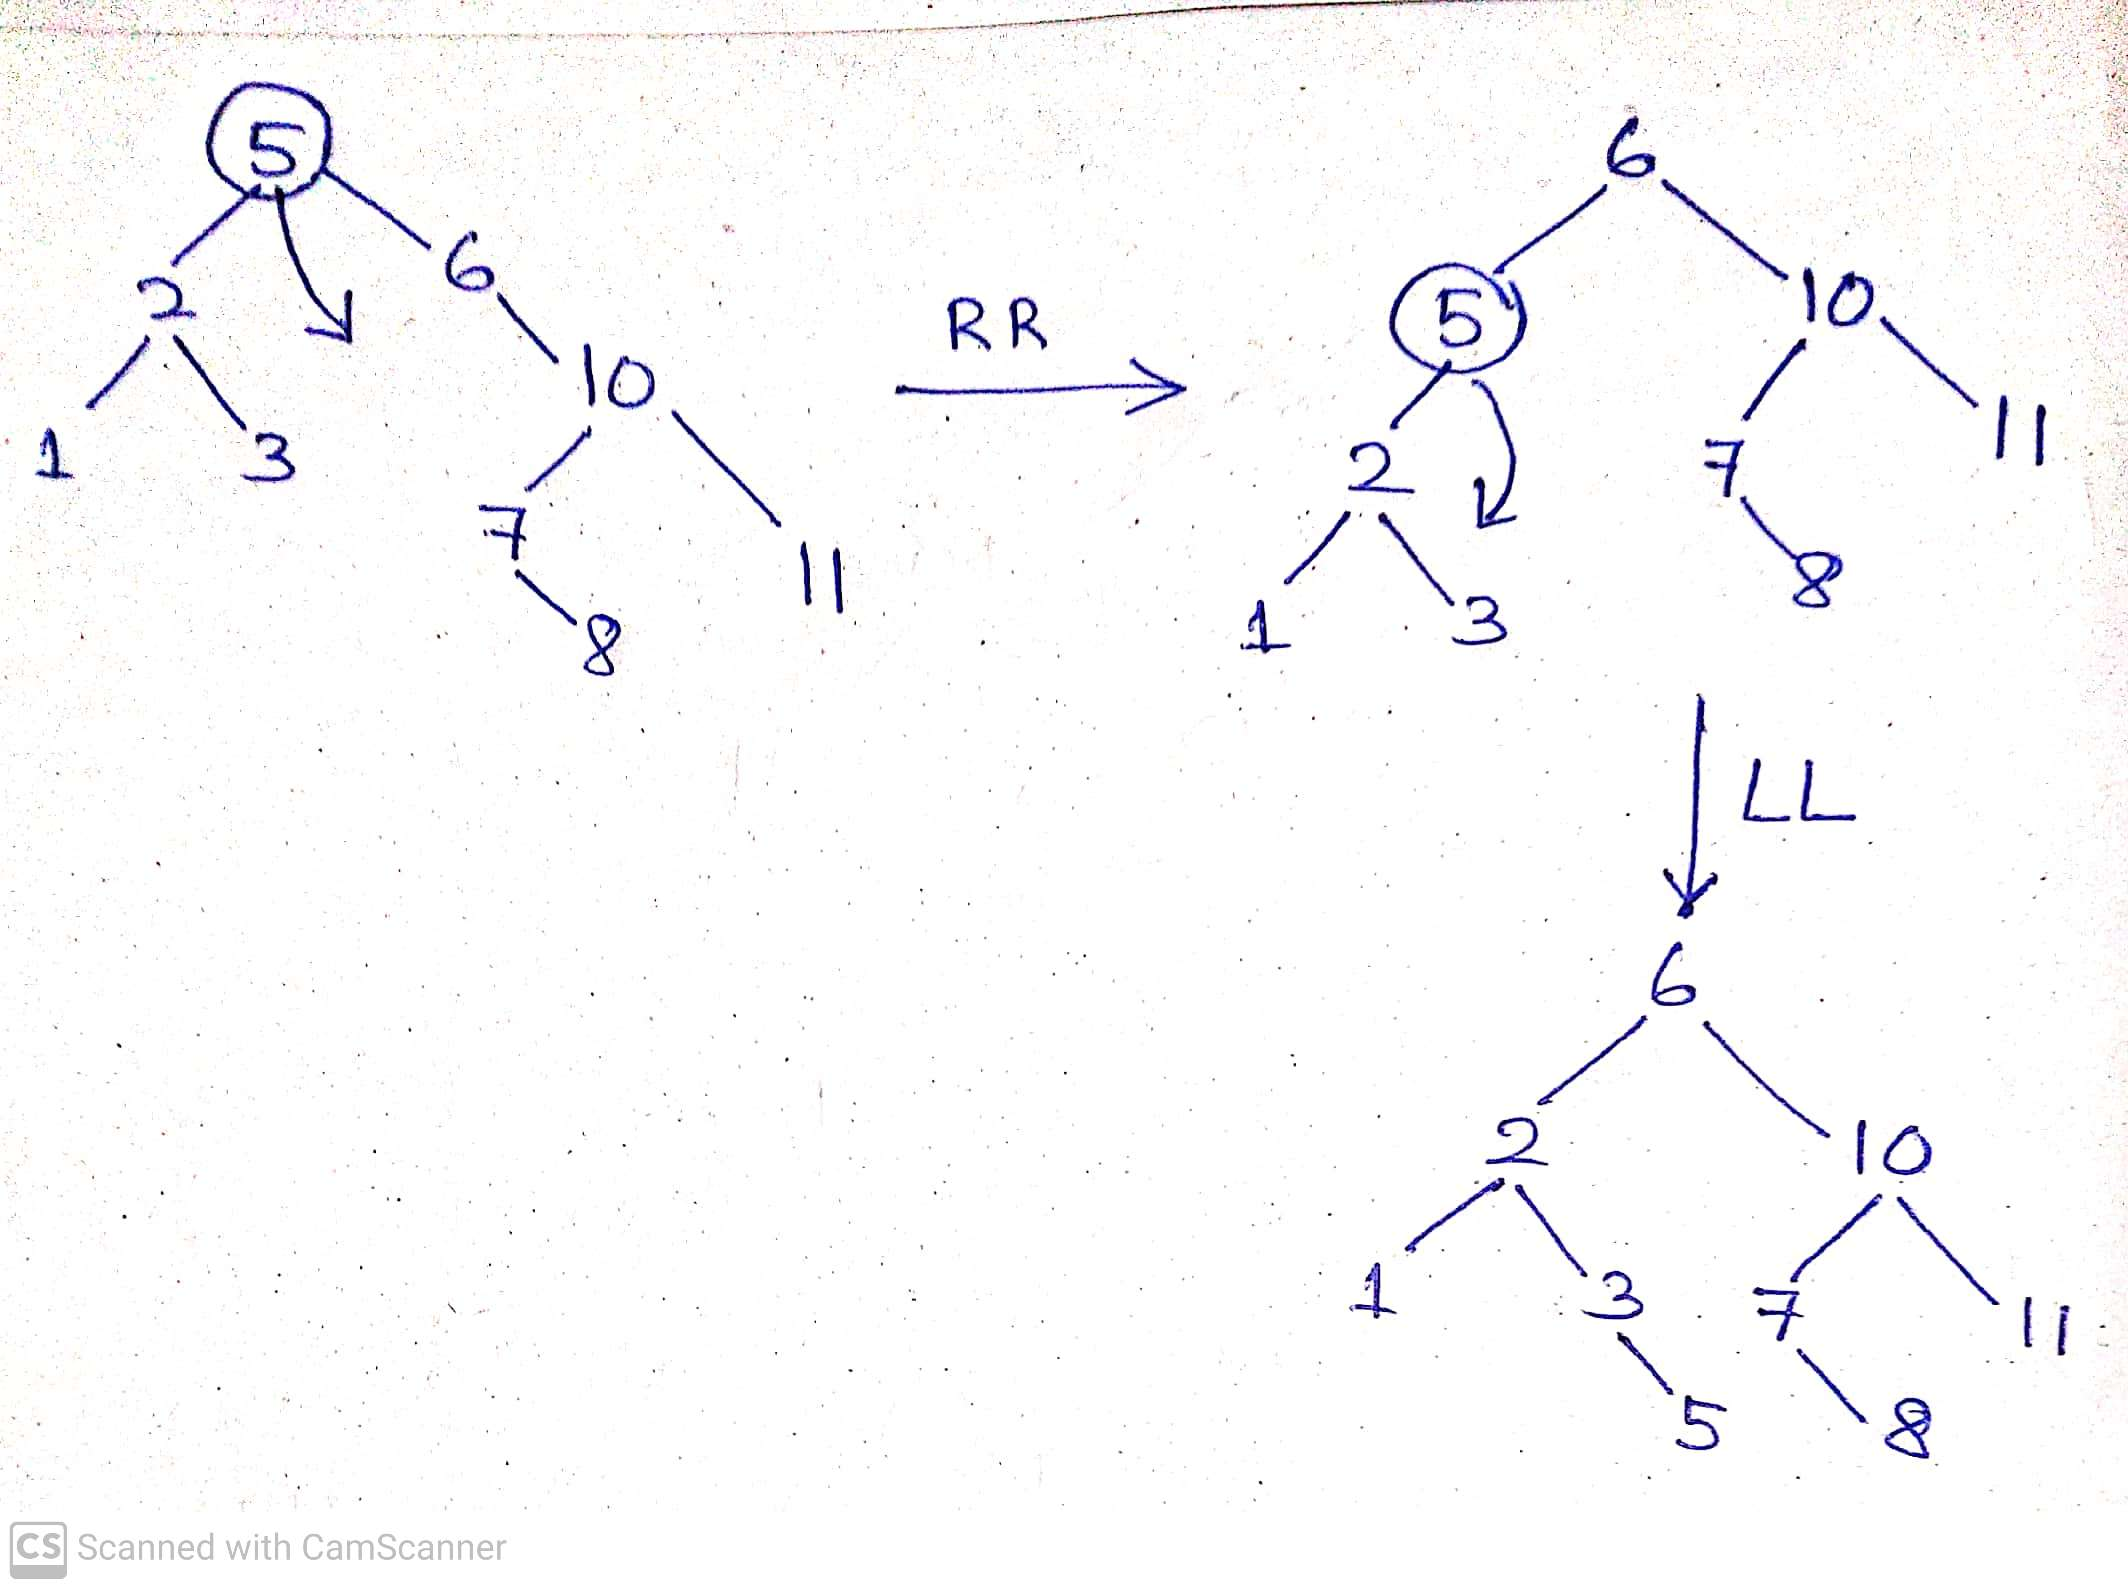
\includegraphics[scale=0.14]{balance2.jpg}\\
		\end{center}

		\subsubsection{Insertion}
		We insert just like a general BST. However, we keep track of the balance factor of the nodes and balance the tree whenever we encounter some unbalncedness(bottome to top). At the end of an insertion, the tree must be balanced.
		\begin{eg}
			Suppose we need to insert the following list in order: 35, 50, 40, 25, 30, 60, 78, 20, 28.
		\begin{center}
			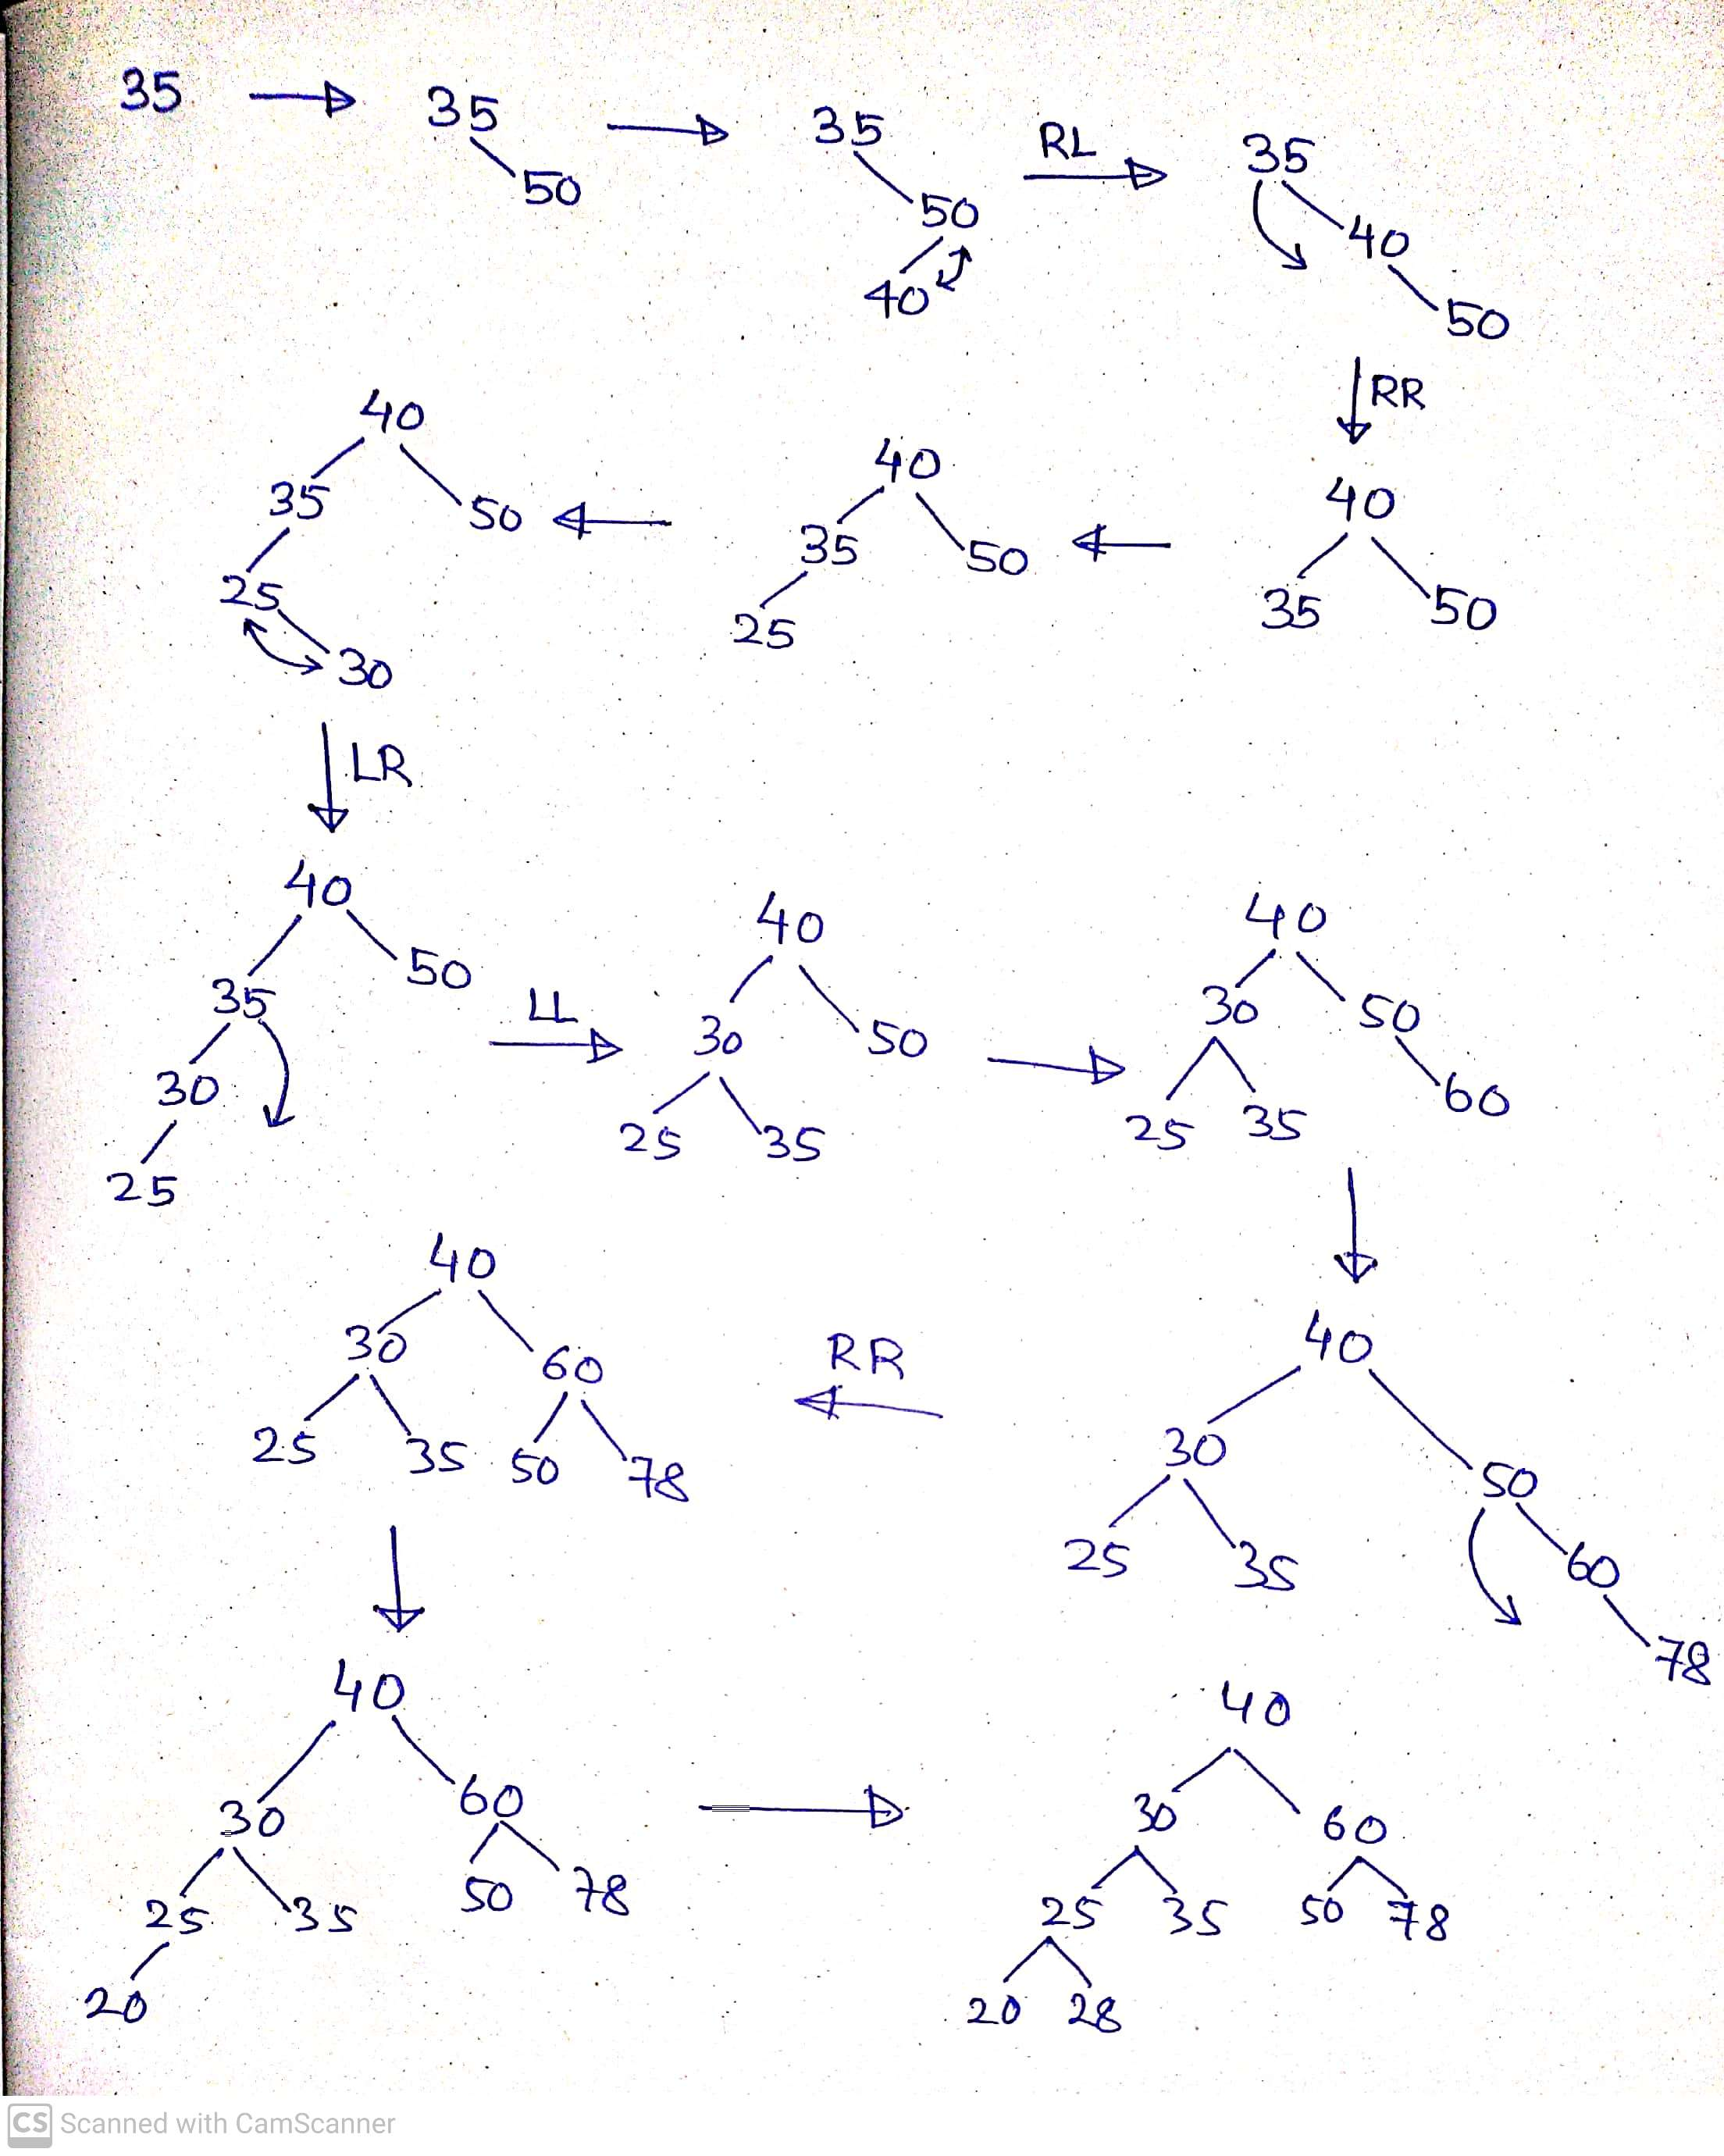
\includegraphics[scale=0.15]{avl-insertion.jpg}\\
		\end{center}
		We required 4 rotations.
		\end{eg}

		As we can see, all operations take $O(\log n)$ time now.

	\subsection{Red Black Tree}
	A red black tree is also a balnced BST. It is somewhat less balanced than AVL search tree, so, search is slower. Red black trees are preferred when we need to do frequent insertions and deletions.
	\begin{defn}[Red black tree]
		A balanced BST with the following features:
		\begin{itemize}
			\item Every node has a colour either red or black.
			\item The root of the tree is always black.
			\item Every NULL leaf is black.
			\item There are no two adjacent red nodes (A red node cannot have a red parent or red child).
			\item Every path from a node (including root) to any of its descendants NULL nodes has the same number of black nodes.
		\end{itemize}
		Every RBT with $n$ nodes has $h\leq 2\log_2(n+1)$.
	\end{defn}

	\subsubsection{Insertion}
	While AVL trees always require rotations to balance, RBTs may require just recoloring of nodes.
	\begin{alg}
			Let X be the newly inserted node.
			Perform standard BST insertion and make the colour of newly inserted nodes as RED.
		\begin{enumerate}
			\item If X is the root, change the colour of X as BLACK.
			\item If X’s parent RED and X is not the root,
				\begin{enumerate}
					\item If X’s uncle is RED (Grandparent must have been black from property 4).
						\begin{enumerate}
							\item Change the colour of parent and uncle as BLACK.
							\item Colour of a grandparent as RED.
							\item Set X = X’s grandparent, Go to 1.
					\end{enumerate}
				\item If X’s uncle is BLACK, do required rotation. After LL or RR rotation, swap the colours of the rotated node and the node about which rotation occured.
			\end{enumerate}
	\end{enumerate}
	\end{alg}
	\begin{eg}
		Suppose, we insert the numbers 10, 18, 7, 15, 16 to an empty tree. Circled nodes are black. 
		\begin{center}
			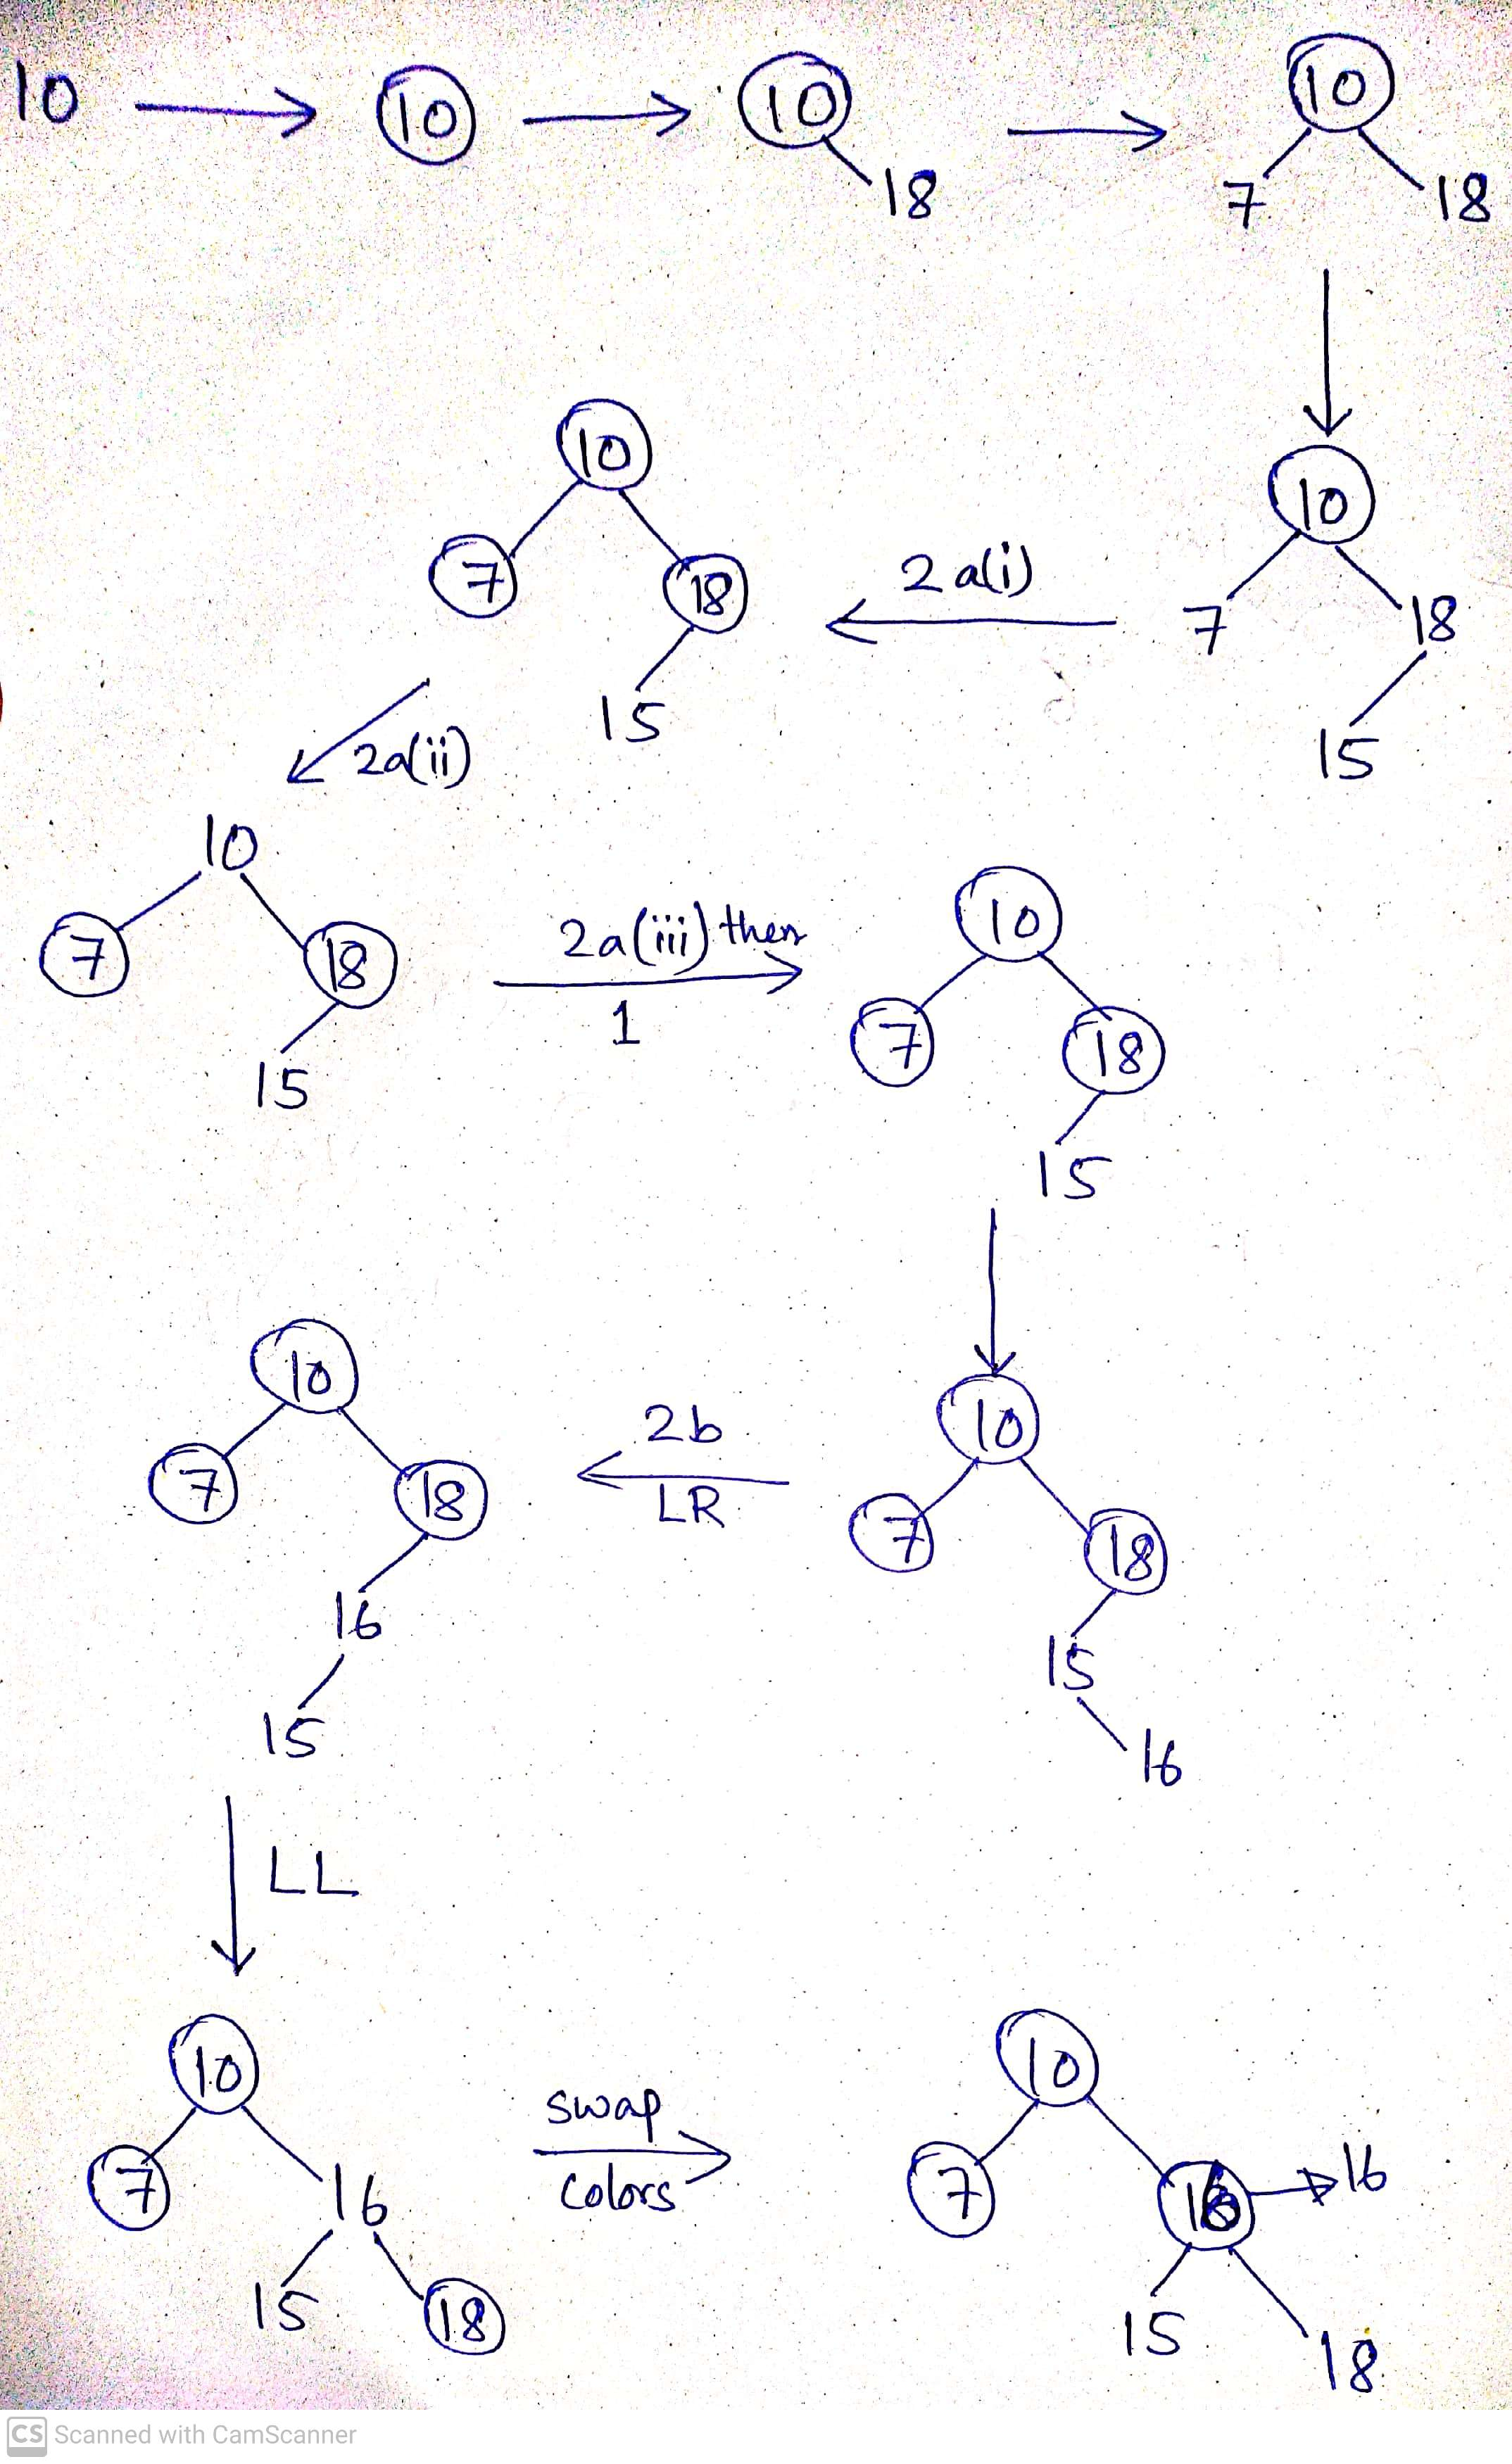
\includegraphics[scale=0.08]{red-black.jpg}\\
		\end{center}
	\end{eg}

	\section{m-way Search Tree}
	\begin{defn}[$m-$way search tree]
		The m-way search trees are multi-way trees which are generalised versions of binary search trees where each node contains multiple elements. Inside a node, elements are in order. The subtree between two keys $k_1$ and $k_2$ contains only keys in the range from $k_2$ to $k_2$.
	\end{defn}
	\begin{defn}[Order]
		The order denotes the maximum number of children a node can have. If the order is $t$, a node can have at most $t-1$ elements.
	\end{defn}
	\begin{itemize}
\item The number of elements in an $m$-way search tree of height $h$ ranges from a minimum of $h$ to a maximum of $m^{h} -1$.

\item An $m$-way search tree of $n$ elements ranges from a minimum height of $log_m(n+1)$ to a maximum of $n$.
\item Operations are similar to BST and require $O(h)$ time.
\end{itemize}
	\subsection{B tree}
	\begin{defn}[B tree]
		A self-balncing $m-$way search tree with the properties:($t$ is the order)
		\begin{itemize}
			\item All leaves are at the same level.
			\item Every node except root must contain at least $\lceil\frac{t}{2}\rceil-1$ keys. The root may contain minimum 1 key.
			\item Number of children of a node is equal to the number of keys in it plus 1.
		\end{itemize}
		Minimum height: $\lceil\log_m(n+1)\rceil-1$\\
		Maximum height: $\lceil\log_t\frac{n+1}{2}\rceil$\\
		Complexity for all operations is $O(\log n)$
	\end{defn}
	The drawback of B tree used for \textbf{dynamic multilevel indexing} is that it stores the data pointer (a pointer to the disk file block containing the key value), corresponding to a particular key value, along with that key value in the node of a B tree. This technique, greatly reduces the number of entries that can be packed into a node of a B tree, thereby contributing to the increase in the number of levels in the B tree, hence increasing the search time of a record.
	\subsection{B+ tree}
	A B+ tree with $l$ levels can store more entries in its internal nodes compared to a B tree having the same $l$ levels.


	\begin{itemize}
		\item The structure of leaf nodes is quite different from the structure of internal nodes.
		\item Data pointers present only at the leaf nodes of the tree.
		\item Leaf nodes store all the key values along with their corresponding data pointers.
		\item The leaf nodes are linked to provide ordered access to the records.
		\item Some of the key values of the leaf nodes also appear in the internal nodes, to simply act as a medium to control the searching of a record.
		\item A B+ tree, unlike a B tree has two orders, $a$ and $b$, one for the internal nodes and the other for the external (or leaf) nodes.
	\end{itemize}
\end{document}
